\chapter{Results}
In the Results section I hope to help the reader understand what I discovered about optimization of reduce neuron models.
How well did it work?
What do these optimized models look like?
And is improving existing published models via optimization possible?

In section \ref{sec:optimizer-verification}, I show how well and under what circumstances the optimizer can work on recovering ground-truth model parameters using simulated data as input.
This is an essential step, since if an model optimized on simulated data does not match the model that simulated it, the whole enterprise can be called into question.

In section \ref{sec:limitations-of-optimization}, I use various suites of biological-data-driven tests to optimize reduced models corresponding to real neuron types.
I show how some of the assumptions and methodological approaches underlying the a subset of the tests might be problematic, and determine their impact on optimization quality. 

In section \ref{sec:optimization-performance} and \ref{sec:optimized-single-neurons}, I assess the quality of these optimizations. 
While I focus on representative cases in this section, an exhaustive account of all optimized models is also available in the Appendix.
I show which models lead to the best fits overall, and for which neuron types.

In section \ref{sec:optimizing-published-models}, I show that most published models actually deviate significantly from biological experimental data.
I locating specific features underlying this disagreement, and explain how this creates an opportunity for optimization to close the gap.
I then show that optimization can bring the behavior of the model and biological neuron back into agreement.

Finally, in section \ref{sec:web-app}, I demonstrate an novel web application for optimization that I created to showcase the work described in the other sections.
This web application can be used to setup, execute, and visualize optimization in real applications or to teach the relevant technical concepts to trainees.

\section{Verification of the optimizer}
Sometimes during optimizer development we used aprior arguments
Four factors needed to be controlled for, before we locate the cause of poor model/experiment fits. Those factors were: the informativeness of measurement errors, the performance of the optimizer, data quality, and model quality.

The digital models we used were known to be not flexible enough to match all electrical features from cell experiments all the time; as compact mathematical functions these models are by nature, self-constrained and therefore they cannot to be fitted to all experimental waveforms. Additionally the data sources may also have some fidelity problems, it was necessary to create data source independent "ground truths", by synthesising plausible data, with the digital models, and optimizing against these ground truths. Because the DEAP genetic algorithm, has been shown to be able solve Rastrigrins function, we expect that our derivative frame work, should be able to fit to simulated data sources, with a high degree of precision, and that is what we found.

The optimizer was capable of producing perfect fits under ideal circumstances. We showed that the measurements the genetic algorithm was using were able to act as informative guides. Since we are confident about the optimizers ability to fit to synthesized data we can then locate sources of model/data disagreement in other places. 

In the subsequent tables and figures when the measurements:time constant, capacitance, Rheobase, Resting potential and Input resistance are used to constrain optimization.
\begin{figure}
    \centering
    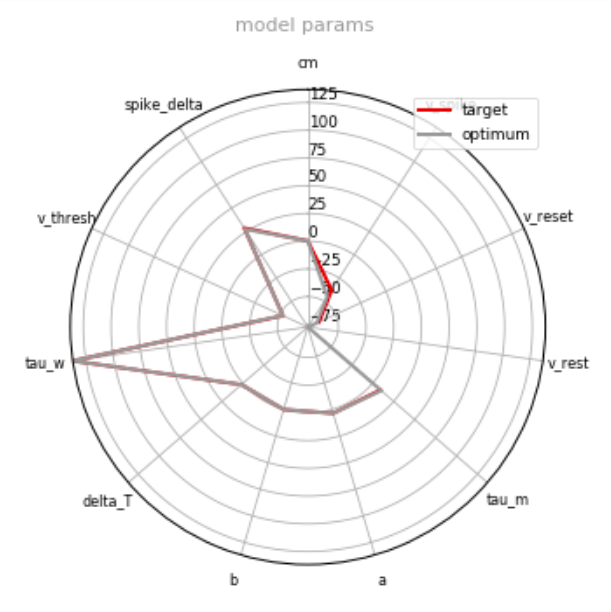
\includegraphics{figures/radar_coordinates.png}
    \caption{This radar plot of model parameters, reveals two mutually inclusive sets, both model parameter values 1 randomly selected, 2 found by the optimizer closely match.}
    \label{fig:my_label}
\end{figure}


%coincide 


\begin{figure}
    \centering
    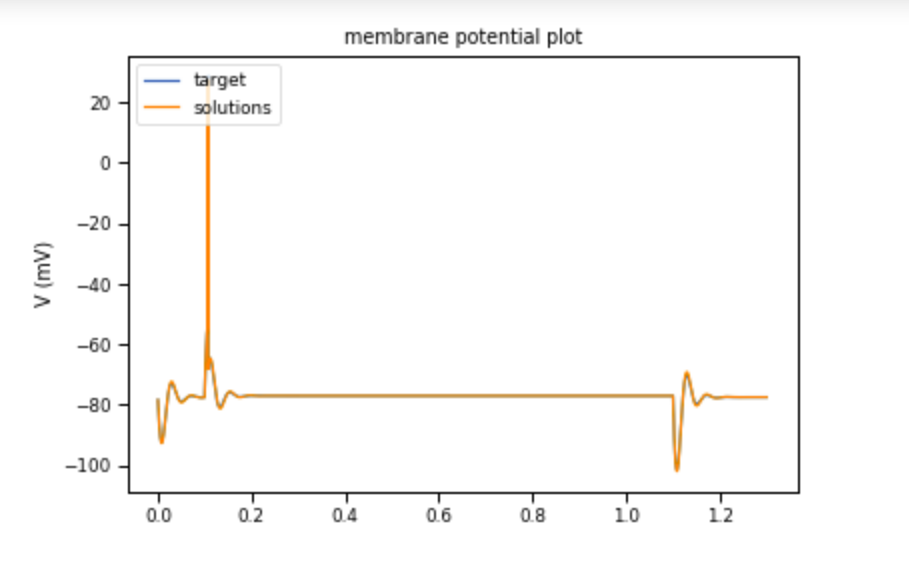
\includegraphics[scale=0.75]{figures/simulated_data_supra_threshold.png}
    \caption{Caption}
    \label{fig:my_label}
\end{figure}
\begin{figure}
    \centering
    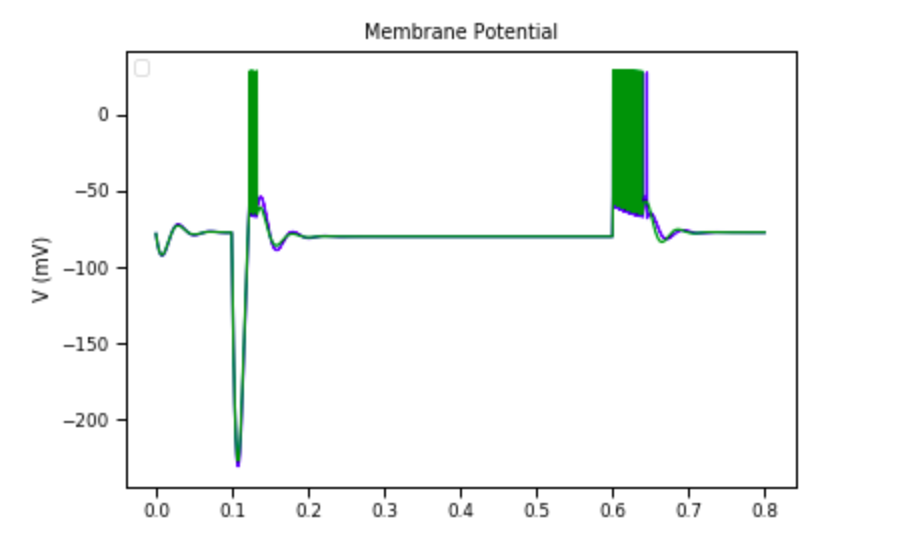
\includegraphics[scale=0.75]{figures/simulated_data_sub_threshold.png}
    \caption{Agreement between a simulated waveform, and an optimized waveform, when both simulated constraint model and optimized model undergo a current injection value of $-10pA$}
    \label{fig:adexp_model_rebound_spike}
\end{figure}

\begin{figure}
    \begin{center}
    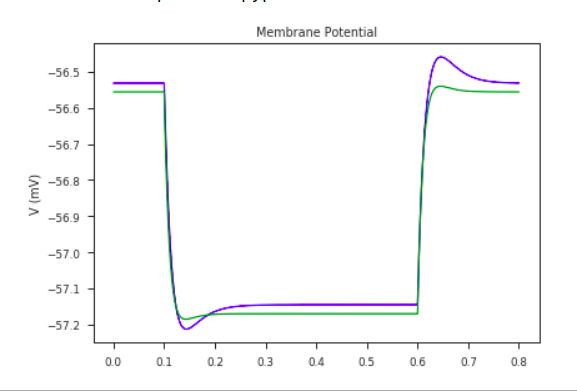
\includegraphics[scale=0.65]{figures/passive_model_agreement}
    \caption{For contrast, this is the Izhikevich model undergoing the same $-10.pA$ current injection value. There is no rebound spike. The model with the blue trace does rebound slightly. Agreement between a simulated constraint waveform, and an optimized waveform, when both simulated constraint model and optimized model undergo a current injection value of $-10pA$}
    \end{center}
    \label{fig:my_label}
\end{figure}

The plot of model membrane potential, as the model undergo's a $-10pA$ current injection, contains multiple spikes in the presence of an inhibitory current is unexpected. The reason this occurs, is because of an unusual model parameterization that makes modelled neuron "rebound spike" in response to attempts to move membrane potential down with voltage.



\ref{fig:adexp_model_rebound_spike}

\begin{comment}

\begin{figure}
    \centering
  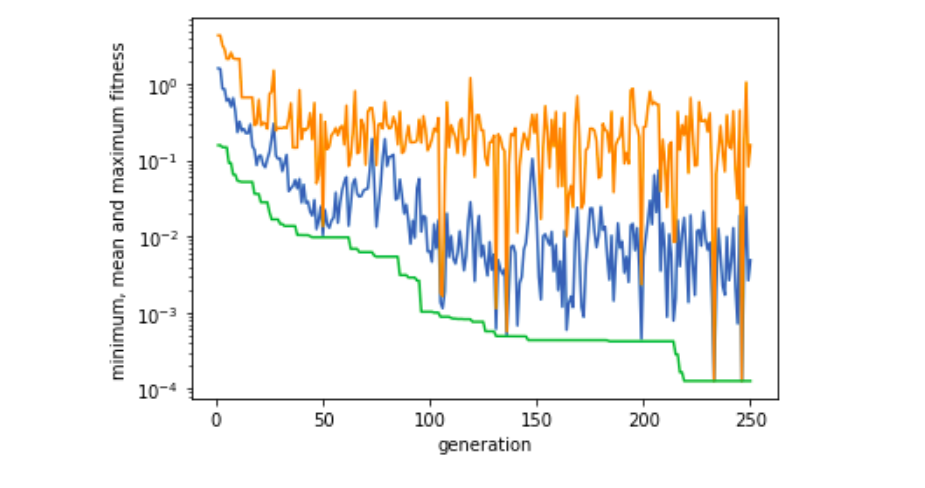
\includegraphics{figures/simulated_data_stats.png}
    \caption{Optimizer evolution, green line tracks evolution of best fitness, blue line average fitness, orange line is worst fitness. GA params, $NGEN=200$, $MU=50$,$cxp=0.3$,$mupb=0.2$ from this plot can see that genes are storing and exploiting information, $cxp+mutpb=0.5$, so $50\%$ of genes are conserved between generations }
    \label{fig:my_label}
\end{figure}
\end{comment}

\begin{figure}
    \centering
    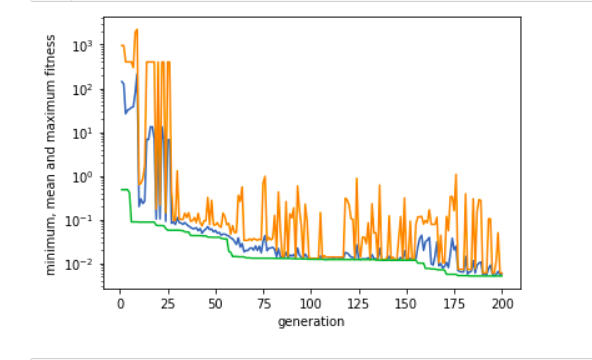
\includegraphics[scale=0.7]{figures/optimizer_internal_validation}
    \caption[Optimizer error over generations]{Optimizer evolution, green line tracks evolution of best fitness, blue line average fitness, orange line is worst fitness. GA params, $NGEN=200$, $MU=50$,$cxp=0.3$,$mupb=0.2$ from this plot can see that genes are storing and exploiting information, $cxp+mutpb=0.5$, a changing number of genes are conserved between generations }
    \label{fig:my_label}
\end{figure}


\begin{table}[ht]
\centering
\resizebox{\textwidth}{!}{
\begin{tabular}{llll}
\toprule
{} &    observations &     predictions & Z-Scores \\
\midrule
RheobaseTest         &         1.62 pA &         1.62 pA &        0 \\
TimeConstantTest     &        13.18 ms &        13.18 ms &        0 \\
RestingPotentialTest &       -77.43 mV &       -77.43 mV &        0 \\
InputResistanceTest  &  270.84 megaohm &  270.84 megaohm &        0 \\
CapacitanceTest      &        48.65 pF &        48.65 pF &        0 \\
FITest               &    7.51 Hz/pA &    7.51 Hz/pA &        0 \\
\bottomrule
\end{tabular}}
\end{table}

AP width, amplitude, and AP threshold errors, did not participate in guiding optimization, because as I have explained, those measurements are not objective between model instances, and thus they lead to misleading error measurements. These tables show that the optimizer can recover ground truths that are derived from simulated data. This result allows us to confidently argue that in fitted models, the cause of model/experiment disagreement must be located in either the data, or the models, but not the optimization process, or the choice of error signals which are demonstrably sound.

%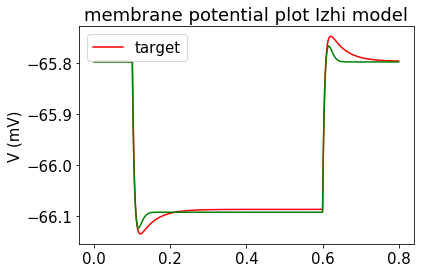
\includegraphics[]{figures/simulated_data_convergence_passive_fits.png}





% probably discussed elsewhere The design of the optimizer used in this work computed rheobase for each model, what that means is a new value of current is required to apply current injection tests to tests that are spiking in nature.\\
%In the optimizer design used here.

%$N-free-model-parameters << N-constraints$
%$(model parameters + %current-injection-value-parameter) << N$ $(independent and uncorrelated)$ constraints.

For the different classes of Reduced Model we show that the optimizer converges when data is simulated.

In a simulated experiment, existing models were instantiated using a randomly chosen model parameters.

The AdExp model, is not an arbitrary waveform generators. Models such as AdExp have intrinsic restrictions that prevent them from matching perfectly with all types of experimental waveforms.


%In the class of reduced neural models we optimized 

When constraints are derived from model measurements, intrinsic model restrictions no longer apply. Optimized models should match perfectly with the simulated experiments. 

* Failure to match is indicative of: -- Failure to setup tractable optimization problems, and under constraining  a high dimensional problem.

- When inverting linear equations, finding a unique solution requires that the number of constraining equations is greater than the number of free variables you are solving for. Analogous to a mathematical technique: Gaussian elimination where unknown variables are solved for using inversion and elimination, in genetic algorithm we solve for unknown variables using stochastic principles, however, underneath implementation details a similar principal exists: Larger amounts of known information can be used to solve for smaller amounts of unknown information. In other words assuming that NOBJ consist of only informative convex error surfaces as a rule of thumb optimization will likely be easy if $NDIM<NOBJ$.

\subsection{Pitfalls}
Choosing optimizer constraints, that cause visible ripples in error surface.
To protect against a situation where the collection of error sources guiding optimization are too correlated with each other, to act as 


\subsection{Verification}
Ground truths are model solutions that we know are correct independently from the optimizer. One way to establish ground truths is to identify the global minima by exhaustively searching the solution space. An exhaustive search is a reasonable approach when you consider only one or two model parameters are free parameters, however if one does 100 samples in each of N dimensions then one must make samples $100^{N}$ total samples to be sure of ehaustively searching, assuming the most efficient code, hardware and development time $N=3$, may be the highs.  Also the choice of 100 samples is nominal, 100 samples could be either too fine or too sparse, depending on how if the parameter being searched exhibits 2nd order sensitivity.

It is more computationally efficient to obtain ground truths by simulating constraining data using digital models. It is easy to simulate constraining data, all that is required is that you take a neuronal model and measure its behavior in response to carefuly chosen current injection values. Measured behavior can then be used to construct NeuronUnit tests, were the measurements become "observations", or observed behaviors. To make the simulated data cover a range of circumstances, one can make different NU measurements by randomly choosing different parameter values of models to find.

It was important to be able to establish ground truths that were always possible for the optimizer to match exactly. Often experimental data implies waveform shapes that are beyond the capabilities of the model that is to be fitted. Simulating experimental measurements meant, that model limitations can be understood separately from optimizer limitations.

 % ie is optimizaation possible?

\section{Limitations of Optimization using Experimental Data}
\label{sec:limitations-of-optimization}

\subsection{When is Optimization Possible Using Real Biological Data?}
Not all of the available data-sets are conducive to optimizing reduced models.
For example, consider the cerebellar Purkinje cell.
The Purkinje cells has a very large surface area (much of it the dendrites that support $~100,000$ synaptic inputs).
It consequently has a large capacitance and a low input resistance, and as such it demands a very large current stimulus to elicit a rheobase spike: $680pA$.
However, most reduced cells typically cannot exhibit such a large rheobase under any parameterization that otherwise looks like a neuron model.
The fact that an expansive dendritic tree is able to absorb so much somatically injected current may be difficult for a reduced model to capture.
Specifically, the upper limit for rheobase found in results was typically as $350-400pA$, but even this comes at the expense of sacrificing fit quality for all other electrophysiological features.
Consequently, optimized models of the Purkinje cell always failed to be biologically plausible.
The p-value of the $\chi^{2}$ statistic was always sufficiently low to reject the null hypothesis that such optimized models were representative of the biological data distribution.
Like the Purkinje cell, the Mitral cells of the main olfactory bulb also escaped successful model fitting.
These mitral cells also have high membrane capacitance $235pF$, and reduced models could not reproduce their features well.  
The Izhikevich model was achieved the lowest overall $\chi^{2}$ statistic for Purkinje cells and Mitral cells, being slightly more flexible than the AdEx or  conductance based models (see Tables \ref{tab:adex-allen} and \ref{tab:izhikevich-allen}).
In general, however, these reduced models may have been developed with smaller, more electronically compact cortical and hippocampal cells in mind.

\subsection{Conflicts between Experimental Features Constraining Optimization}
Feature values extracted from multiple data sets appeared to be in conflict for some cell types.
For example in the section below I show that the rheobase value was often incompatible with some passive electrophysiological feature values, such that good optimization could be achieved with one set or the other, but not both together.

\subsubsection{Tradeoff Patterns in Data-driven Tests in Subtheshold and at Threshold Electrical Properties}
\label{sec:rh_incomp}
Using data from the Allen Cell Types neuron with ID $471819401$,
I was able to optimize both AdEx and Izhkevich models, such that both models would agree with rheobase, time constant, resting membrane potential, and input resistance, experimental values. Some tradeoffs were needed in order match all of the values, as these features could not all be perfectly matched at once.
\begin{table}
\begin{center}
\begin{tabular}{|l|l|l|l|}
\toprule
Test name &   observations &    predictions & Z-Scores \\
\midrule
RheobaseTest         &       190.0 pA &      199.52 pA &     0.04 \\
TimeConstantTest     &        13.8 ms &        6.21 ms &     0.32 \\
RestingPotentialTest &       -77.5 mV &      -39.29 mV &     0.26 \\
InputResistanceTest  &  132.0 megaohm &  44.94 megaohm &     0.45 \\
\bottomrule
\end{tabular}
\caption[AdEx model fit quality]{Predicted and observed features for neuron $471819401$ from the Allen Cell Types database, following optimization of the AdEx model against data from this neuron.
Other neurons showed similar optimization performance, and are shown in the Appendix.}
\label{tab:adex-allen}
\end{center}
\end{table}

\begin{table}
\begin{center}
\begin{tabular}{|l|l|l|l|}
\toprule
{} &   observations &    predictions & Z-Scores \\
\midrule
RheobaseTest         &       190.0 pA &      190.48 pA &        0 \\
TimeConstantTest     &        13.8 ms &         1.9 ms &     0.94 \\
RestingPotentialTest &       -77.5 mV &      -70.65 mV &     0.03 \\
InputResistanceTest  &  132.0 $M\Omega$ &  25.47 $M\Omega$ &     0.74 \\
\bottomrule
\end{tabular}
\caption[AdEx model fit quality]{Same as the Table \ref{tab:adex-allen} but for the Izhikevich model.}
\label{tab:izhikevich-allen}
\end{center}
\end{table}

%And different specimen id's For example: 482493761 id:
%Adex:
%\newline
%\begin{center}
%\begin{tabular}{|l|l|l|l|}
%\toprule
%Feature Name &   observations &               predictions & Z-Scores \\
%\midrule
%RheobaseTest         &        70.0 pA &                   73.4 pA &     0.04 \\
%TimeConstantTest     &        24.4 ms &  0.0029 ms &     9.32 \\
%RestingPotentialTest &       -71.6 mV &                 -49.76 mV &     0.13 \\
%InputResistanceTest  &  132.0 megaohm &             72.15 megaohm &     0.23 \\
%\bottomrule
%\end{tabular}
%\end{center}
%\end{table}


%Izhikevich:
%\begin{table}
%\begin{center}
%\begin{tabular}{|l|l|l|l|}
%\toprule
%{} &   observations &    predictions & Z-Scores \\
%\midrule
%RheobaseTest         &        70.0 pA &       71.19 pA &     0.01 \\
%TimeConstantTest     &        24.4 ms &        2.85 ms &     1.05 \\
%RestingPotentialTest &       -71.6 mV &      -55.05 mV &      0.1 \\
%InputResistanceTest  &  132.0 megaohm &  46.06 $M\Ohm$ &     0.43 \\
%\bottomrule
%\end{tabular}
%\end{center}
%\end{table}


%\begin{table}
\subsubsection{6239608801 AdEx}
The need to match the rheobase appeared to be interfering with the ability of the optimizers to match many other features.
The rheobase is essentially the knee of the FI curve.
An alternative strategy is to produce models that match the slope of the FI curve.
Here I show two out of $12$ examples demonstrating that that fitting models to the FISlope and rheobase only, leads to generally better agreement as there is less conflict between these two tests.
%\textbf{Model Parameters}
%\newline
%\begin{center}
%\resizebox{0.7\textwidth}{!}{
%\begin{tabular}{|l|r|r|r|r|r|r|r|r|r|r|r|}
%\toprule
%{} &          cm &    v\_spike &    v\_reset &     %v\_rest &      tau\_m &         a &         b &   delta\_T &       tau\_w &   v\_thresh &  spike\_delta \\
%\midrule
%0 &  147.166079 & -45.027618 & -32.175811 & -51.521467 &  51.323969 &  1.787643 &  5.553571 &  4.143261 &  158.661633 & -25.749411 &    15.471554 \\
%\bottomrule
%\end{tabular}}
%\newline
%\end{center}
%\end{table}

\begin{table}
\begin{center}
\begin{tabular}{|l|l|l|l|}
\toprule
{} & observations &   predictions & Z-Scores \\
\midrule
FITest       &   0.18 Hz/pA &  0.18 Hz/pA &     0.01 \\
RheobaseTest &      70.0 pA &      70.26 pA &        0 \\
\bottomrule
\end{tabular}
\end{center}
\end{table}

\begin{table}
\begin{center}
\begin{tabular}{|l|r|}
\toprule
chi\_square &  0.000083 \\
p\_value    &  1.000000 \\
\bottomrule
\end{tabular}
\end{center}
\caption[Quality of Fit to Experimental Data]{Summary statistics of fit quality using AdEx model, when it is constrained against FITest, and Rheobase Test alone.
The very low $\chi^2$ statistic (and high p-value) indicate that there was no evidence that this optimized cell model produced behavior outside of the range of biological neurons of the same type, at least for the features examined here.}
\label{tab:chi2-p-1}
\end{table}

%\newline

\subsubsection{6239608801 Izhikevich}

%\newline
%\textbf{Model Parameters}
%\newline
%\begin{center}

%\begin{tabular}{|l|r|r|r|r|r|r|r|r|r|r|}
%\toprule
%{} &           C &        k &         vr &         vt &      vPeak &        a &          b &          c &          d &  celltype \\
%\midrule
%0 &  190.848367 &  0.77007 & -65.461028 & -49.496538 &  31.461532 &  0.05877 &  13.916167 & -58.159122 &  38.738638 &         7 \\
%\bottomrule
%\end{tabular}}
%\end{center}


\begin{table}
\begin{center}
\begin{tabular}{|l|l|l|l|}
\toprule
Features & observations &   predictions & Z-Scores \\
\midrule
FITest       &   0.18 Hz/pA &  0.18 Hz/pA &        0 \\
RheobaseTest &      70.0 pA &      66.61 pA &     0.04 \\
\bottomrule
\end{tabular}
\end{center}
\begin{center}
\begin{tabular}{|l|r|}
\toprule
chi\_square &  0.00155 \\
p\_value    &  1.00000 \\
\bottomrule
\end{tabular}
\caption[Quality of Fit to Experimental Data]{Similar to Table \ref{tab:chi2-p-1}, but for Izhikevich model. Since two major model classes are better able to fit to FITest and Rheobase alone, it suggests that these two measurements might be less conflicted in models.
}
\end{center}
\end{table}


By ``good optimization" I mean that the optimized model exhibited behavior that was consistent with all of the features.
Models seemed to have particular difficulty in recapitulating an accurate fit for rheobase, while simultaneously satisfying the fitness criteria imposed by the time constant, input resistance, capacitance and resting membrane potential.
This was less problematic when using the slope of the FI curve as a feature, suggested that it was not spiking \emph{per se} that caused the problem.

This was also evident when working across datasets.
For example, when optimizing against data from both NeuroElectro and the Allen Cell types database, it was typically impossible to satisfy data-derived features from both sources simultaneously, even when the same nominal neuron type was being described.

%The l5pc model was pre-optimized to fit to spike times and F/I mainly, and so it should not necessarily be expected to fit other electrical characteristics of the cell. Only the rheobase test, and the time constant test seemed to fall within the range of biological plausibility. None the less, this model remains a useful benchmark for reduced neuronal models.
%It was desirable to include this extended range of Izhikevich model behavior
%However, as noted in the introductory material, it i 
%Previously I mentioned neuronal modelling competitions I have optimize every model against the same data sets in order to assess overall which model is better able to fit to diverse data sets.

%
%\begin{comment}
%\subsection{Neocortical Layer 4/5 Pyramidal Cell Test Suite}
%\subsection{%2a}
%Direct Quote: "widening of the spike shape, decrease of the firing rate and change in the interspike interval distribution". %All these single unit waveform shapes increased their width with temperature.\cite{goldin2017temperature}

%1a/b Is Optimization possible?
%       1a. Construction of tests from diverse experimental sources (I wrote the neuroelectro api and its use in neuronunit, and wrote the original Allen one, but you have put in work to create runnable tests from these and other sources).  This is in a sense a method, but you can still report that these tests are runnable, even outside of optimization.
%       1b. Simulated data tests of optimization.  What works?  What doesn’t?  Why (briefly, saving some for discussion)?  NeuroElectro vs Allen also belong here, and fits in with 1a.  You should talk about model means vs means of models (or whatever we are calling it) here, if you have the results for it or think you can in 3 weeks.  
       %You can talk about rippled error surfaces — this is such a deep technical detail that I wouldn’t spend a lot of time on it.  In other words it may be important but it will be almost impossible to follow even if written well.


%During optimization knowledge of error surfaces should not be mandatory but it can help to solidify good optimization outcomes.  Through human examination of resulting error surfaces, it was found that some of the novel test sets were not helpful to the optimization framework.  Interestingly some types of tests had a propensity to amplify errors originating from elsewhere.

% depended on current stimulus values that were not fixed between models, but instead where contingent on the changeable state of the model cell, this measurement was usually the derivative of membrane potential: $max(\frac{dV_{m}}{dt})/10$. For more on this see \ref{sec:Optimization Pitfalls} 
% duplication
%I found that some fraction of these new tests were because they depended on measured features relative to some other changeable measurement inside the cell usually $max(\frac{dV_{m}}{dt})/10.$ As I discuss in methods, had the propensity of amplifying errors that propogated from elsewhere. 
%This required both the extraction of novel features [EFEL: ISI, AHP-depth, adaption ratio etc.] on new data types types.

%This class was also acculated useful helpful methods such as retrieving default model parameters.



%Flat regions of error surface are uninformative.
Tests that the author curated from Allen Cell types led to some models being under-constrained about spike width. The severe consequences of under-restraining were not obvious, they were revealed by graphs in a virtual experiments were appropriate models were elicited to spike. The lack of constraint was easily rectified, by imposing a specific spike width constraint on Adaptive exponential models, however, unexpectedly in this context, the models $\chi^{2}$ increased dramatically and biological plausibility plummeted, in all except one test. To  paraphrase, the adaptive exponential models had found an unexpected way to cheat tests, by taking advantage of a lack of constraints in an unrelated area.



There was a need to create extra constraints for fitting models, as the set of Allen Constraints was too few in extent, and not sufficient to properly constrain models.



In type of standard, the NeuronUnit tests, themselves act as the final judge of model quality, in the absence of a spike width tests, many AdExp models were able to get very good fits on against supplied constraints, but plots of actual spike shape looked very unnatural, as spike width lasted $>=$ 6ms. Applying extra standards beyond the NeuronUnit tests creates a dilemna. As all the GLIF models, presented unusual spike shapes.


\subsubsection{Experiment Fitted Model Results} 

%Allen Brain Institute, Cell-types E-Physiological data, Elephant Tests
%\subsection{Experiment Fitted Results Neuroelectro data, Elephant Tests}

Over four different Allen experimental sweeps, and four different different cell type specific electrical observations, we created eight unique data sets, and then converted these eight data sets to neuronunit test suites.

We then took four different models, and we attempted to fit each test set to each model. The result of was a four $\times $ eight factorial of model data combinations. For each each member of this 32 set factorial we wanted to know if the fitted model behaved in a biological plausible manner, we were interested to know if fitted models were convincing mimics of in-vivo cells, at least with respect to the measurements models were trained to fit.


\subsection{Standard Error of the Mean}
\begin{tabular}{lrrrrrrr}
\toprule
{} &  Rheobase &  SpikeThreshold &  SpikeHalfWidth &  SpikeAmplitude &  MembraneTimeConstant &  RestingMembranePotential &  InputResistance \\
sem                                &           &                 &                 &                 &                       &                           &                  \\
\midrule
Hippocampus CA1 pyramidal cell     &    122.88 &            1.85 &            0.12 &            3.68 &                  3.88 &                      0.72 &            12.57 \\
Olfactory bulb (main) mitral cell  &       NaN &            5.69 &            0.12 &            2.83 &                  5.42 &                      1.39 &            20.17 \\
Cerebellum Purkinje cell           &    419.81 &            2.00 &            0.05 &            0.57 &                   NaN &                      3.69 &            19.26 \\
Neocortex pyramidal cell layer 5-6 &    128.87 &            1.92 &            0.17 &            1.49 &                  2.56 &                      1.84 &            27.93 \\
\bottomrule
\end{tabular}


Since some of the NeuroElectro data sources were more challenging to fit, we also computed the Standard Error of the Mean, so that later we could interprite model fitting failure. Forinstance, the SEM is a prediction of a measurements dispersal, it is often used when the standard deviation is unknown. 

The $\chi^{2}$ statistic, and the p-value give us a formally indicates how convincing each fitted model was in its mimicry of biological measurements.
Because we already have a list of Z-scores, the $\chi^{2} $statistic can be obtained by squaring each Z-score and summing the result. A sum of squares less than 1, tells us that models performed well.
$\chi^{2}=\Sigma_{i} (Zscore_{i}^{2}) $

%https://en.wikipedia.org/wiki/Chi-square_distribution
%This allows you to state this as a hypothesis test with a p-value.  The chi-square statistic would simply be , and the p-value would be 1-scipy.stats.chi2.cdf(x, 8) where 8 is the number of elephant tests (and Z-scores).  A very small p-value (which would come from very large chi-square statistic, much larger than expected for random variation) %would mean the optimizer was less successful at recovering the true model.

See appendix:\ref{table:static_electrical_properties}
The Izhikevich Model and the Point Conductance Model were able to achieve high p-values, and small chi-squared statistics when seven or eight of the tests were considered together.

For example the Izhikevich model fitted to Hippocampus CA1 pyramidal cell data achieved $ (\chi^{2} ,p-value) =(2.1250913868824415, 0.9769347643323284) $

The olfactory Mitral cell
$ (\chi^{2} ,p-value) =(2.0190436240810925, 0.9804224622781068) $

and the cerebellum Purkinje cell. For contrast p-value and chi-squared statistics on the best random models were:

%(2.0190436240810925, 0.9804224622781068)r
\subsection{Data fitted Results on four different classes of model were only modestly good for the Izhikevich Model and the Point Conductance Model}

To make the argument that limitations in reduced neural models were the cause of modest model/experiment agreement, we first had to rule out alternative possibilities. One possibility was that the experimental measurements were faulty, and that the measurements were possibly spurious because of in appropriate averaging. It was found that mainly the olfactory bulb mitral cell was prone to having underlying bi-modal data distributions, and this was especially true for resting membrane

that the models shouldn't be able to reproduce. When considering the data sources, the methods of data collection and data quality should be reliable, the one main 

we first needed to exclude the possibility that there might be something wrong with the data, we are fitting models to.

We needed to rule out was that the data sources did not reflect bi-modal distributions, since the neuroelectro data was the actually the mean over different laboratories, animals, and recording epochs. The mean of a population can often be a robust representation of a population, however there are circumstances when the opposite is true, such as when the underlying data is generated by two different processes, leading to bimodal distributions. Fortunately, it is not hard to test if experimental data, has an underlying bimodal distribution. That test was performed using human judgement for all measurements that were used to fit the model to experiments. Except in the case of the Allen Brain data, because the Allen Brain data consisted of individual raw experiments, and population averaging did not apply. For measurements used in the elephant optimization pipeline.

Below I show distributions for  Time Constant, Input Resistance, Capacitance, Rheobase, Resting Membrane Potential, bimodal distributions did not apply, so we could rule out inaccurate data as a reason for poor model performance.

There is no reason to believe that reduced neural models could not be made to fit inaccurate neural recordings as well as real ones, if the fiction is just caused by noise, then it is still possible that hypothetical spurious values would still be in reach of the Izhikevich model. The izhikevich model can be made to generate some physiologically implausible waveform shapes. 
% a different question, of are the models arbitary waveform generators? 

Besides even if the data was wrong, it wouldn't necessarily follow that models couldn't reproduce the inaccurate data. Instead what we see is, that models can fit one type of experimental measurement at a time, but they can't fit all measurements at once. This result suggests that model flexibility is the most fundamental cause of modest, model experiment disagreement.


%In light of this result, one might ask, i
If reduced models are not excellent at fitting data, are brain simulations really that much more realistic, when we use data driven fitted models in the place of generic model parameters? If data driven model fits lead to models that fit one measurement better than others, which fitness criteria will lead to the greatest consequence for network simulations?

%to answer that question we have created some large




\section{Limitations data we were using was of Existing Approaches} 
Existing community supported simulated models were problem ridden, and our own custom methods were used as work arounds.

% NEURON version of Izhi model is not as fast as one might expect, this may because of the way we tried to implement the model, by creating and destroying HOC module instances, that contain the model. 

%A
% Nonetheless, 
At first we accessed an implementation of the Izhikevich model that was translated from jNEUROML into a NEURON simulator implementation. The problem with this implementation is that it had fragmented the whole Izhikevich model into chattering and non chattering subtypes. The model implementation seemed to have an internal conflict between two capacitive terms. The problem was that the Izhikevich model requires only one capacitive term.

implemented in NEURON which was derived from a J-NeuroML translation, could not reproduce all of the Izhi original publication figures, because it had two different conflicting sources of capacitance.\\
\\
From J-NeuroML we created NEURON version of Izhikich model, however we were not able to make this model execution times brief enough to be useful for optimization. Although the NEURON simulator is designed to be fast, their may be a cost associated with reloading the NEURON environment many times in fast succession.

This should not go in the general introduction, but in the intro to the appropriate section of the results where you use those models. 
\subsection{Does an Averaged Model Recapitulate Averaged Measurements?}
For a selection of three model measurements:

We are interested in the question: ``Could misrepresented data, lead to a situation were models try too hard to match targets that the models were not built to explain?" %We were interested in the consequence of this worst case. 

I placed two different versions of the same  model class in different locations of parameter space. For each location I measured: rheobase, input resistance, capacitance, and membrane time constant.
I then averaged these measurements together to obtain a mean set of electrical measurements, its this collection of measurements that I refer to as "mean measurements". Next we created a "mean model' by averaging the locations in parameter space together.
In averaging between two points we create a third point that is midway between the pre-existing coordinates. I refer to the third midway point as a "mean-model".
The mean model is used to create a third set of model measurements, as we are really interested in the question: "Does the mean model sometimes fail to recapitulate the mean measurement?"


%With these different parameter sets we took separate measurements of the listed electrical properties, 
When we have mean measurements, and also mean model measurements, it enables us to understand if bi-modal distributions of measurements in experimental data can pose a problem for optimization of cells.

Previously in methods \ref{section:nelectro}, we graphically inspected the neuroelectro data sources closely, in order to assess each measurements distribution.
We revealed Bi-modal distributions in input resistance, and cell membrane capacitance, but we do not yet know if it is invalid to fit to the mean of a bi-modal distribution.
Consider a  cell class which had an underlying bimodal distribution for input resistance. An individual cell from this class produced measurements for input resistance midway between two modes for input resistance.
Its entirely conceivable that that this mean cell would produce measurements that were also the mean of the two modes, however, we cannot assume that there this to be true, it seems equally likely that this midway cell produces a measurement for input resistance, that is significantly higher or lower than the mean of the two modes. To bolster that this non linear behavior could be a problem with in-silico models of in-vivo experiments.
We created virtual experiments to expose non-linear behavior between two  close, but different sets of model parameters.

%set about establishing that it is a problem in modelling space.
%The genetic algorithm approach, of recombining model parameters to sample error surface is a similar concept. We do not naively interpolate using midway points, becuase we don't expect that small changes in model parameters to have linear effects.
%to sampling models 

We expect the Izhikevich model, and the adaptive exponential models to support ``regime" change, that is we know that there are regions in parameter space that where when entered cell behavior becomes fundamentally different. For instance in the Izhikevich model, some regions support tonic-bursting and other regions support chattering. 

\begin{figure}
    \centering
    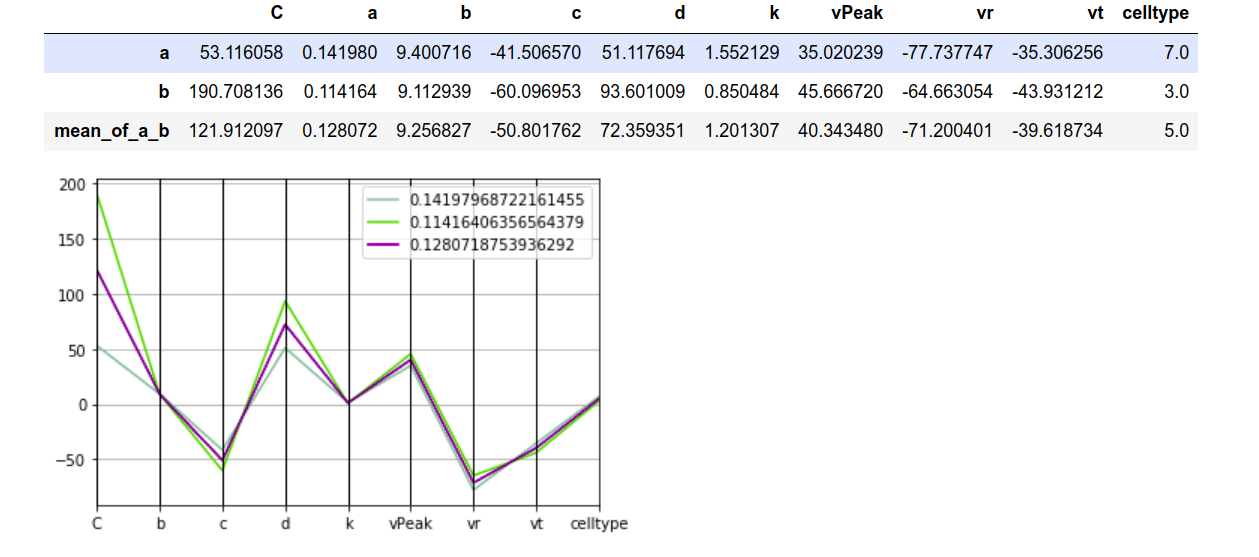
\includegraphics{figures/mean_model_mean_measure_ment_params.png}
    \caption{Caption}
    \label{fig:my_label}
\end{figure}

\begin{figure}
    \centering
    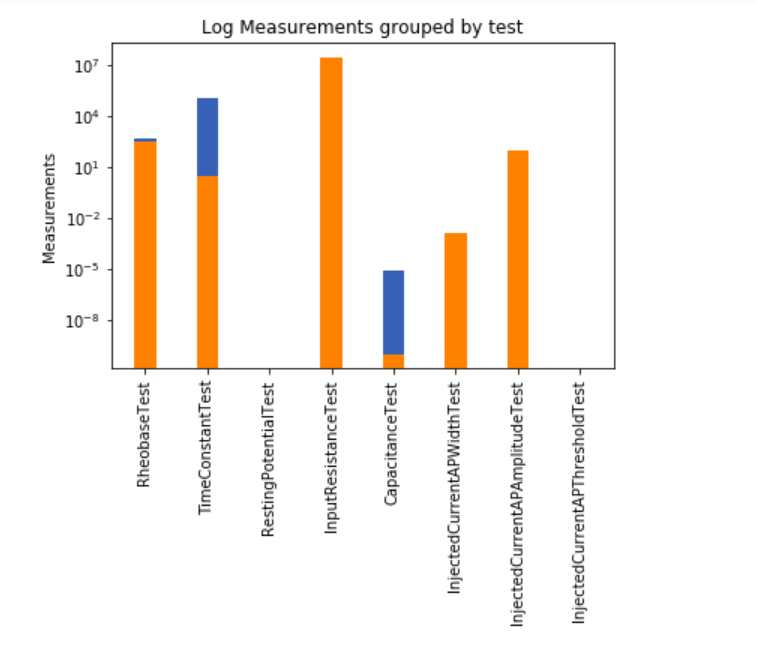
\includegraphics{figures/mean_model_mean_test.png}
    \caption{Caption}
    \label{fig:my_label}
\end{figure}

\begin{figure}
    \centering
    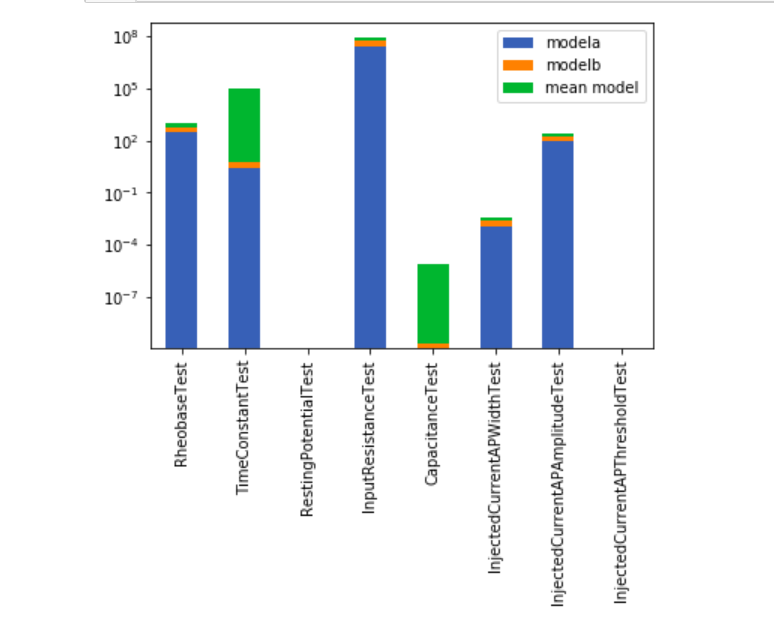
\includegraphics{figures/mean_model_mean_test2.png}
    \caption{Caption}
    \label{fig:my_label}
\end{figure}

explore if this was a problem for models as well as experimental cells.
%Previously, the INCF hosted a model data fitting competition, were participants competed to submit models that %were best able to fit membrane voltage from a variety of above-threshold current injection experiments see %figure \ref{fig:}. In this competition, unlike in this work the best models had to predict spike time. Within %the scope of this project, post-optimization, ranking of the different models in terms of their ability to %explain the most in-vivo experiments.  There are some data sources, that no models seem to do well on, however, %the majority of experiments cause good fits, and the models should compete with each other.
%\subsection{Neocortical Layer 4/5 Pyramidal Cell Test Suite}

%Direct Quote: "widening of the spike shape, decrease of the firing rate and change in the interspike interval distribution". %All these single unit waveform shapes increased their width with temperature.\cite{goldin2017temperature}



%\subsubsection{%\subsection{Section 2.1}
%
%2. Results for several optimized models.
%    2a. First just do basic ones (like Izhikevich) for a few cell types, then you can close with L5PC.
%    2b. The app (which supports 2a).

%\subsubsection{2a}

\section{Performance of Optimized Models}


\subsection{Somatosensory Layer 5 Pyramidal Neuron Model Applied to NeuronUnit Data Driven Tests}

Below I introduce a different approach to parameter fitting work: a multi-compartment, conductance based layer 5 pyramidal cell model \citep{van2016bluepyopt}, was appropriated from BluePyOpt optimization framework, and massaged into the NeuronUnit framework.
This model subserved as one of many component neurons in the original formulation of the Blue Brain Project \cite{markram2015reconstruction}.


This elaborate biophysical model is the philosophical opposite of the reduced models focused on in the majority of this thesis work, since the model incorporates electrically complex phenomena instead of excluding it from the model.
The complex model includes a dendritic action potential which can travel ``backwards" from distal dendrite to soma where it is free to summate with incoming EPSPs.
As you can see in the list of parameters (Figure \ref{fig:ca1_parameters}), The model has different adjustable conductance's in 3 out of 4 membrane domains including axons, dendrites, and soma. In the figure \ref{fig:brief_shape} you can membrane zones with different channels are color coded: apical dendrites (magenta), basal dendrites, and axons.


\begin{figure}%{.2\textwidth}
  \begin{center}
    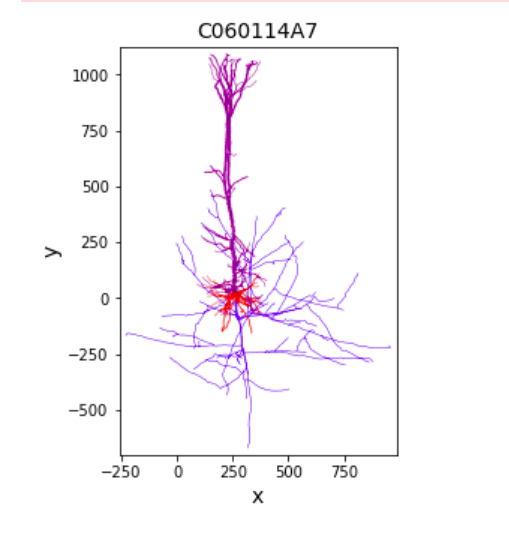
\includegraphics[scale=0.8]{figures/morphology_view.png}
    \caption[l5 pyramidal neuron tree]{This l5 pyramidal neuron model is spatially extended, so a 2D depiction of its dendrite and axonal tree is warranted.}
  \label{fig:brief_shape}
  \end{center}
\end{figure}


There are also other parameters (not displayed here) which are fixed, but those specified in Figure  \ref{fig:ca1_parameters} are amenable to fitting in the context of optimization.


An existing cell from the layer 5 somato sensory rat, hind leg region was acquired by cloning an the BluePyOpt GitHub Repository \cite{van2016bluepyopt}.
Neuroelectro lumps together, prefrontal cortex, somatosensory cortex and V1 PC cells together into a generic frontal cortex pyramidal cell model. 

% Overall it seems

%on NeuronUnit tests of model data agreement}
%\subsection{Section 2.1}
%
%, so it is probably not comparable to NeuroElectro Data.
A suite of neuronunit tests containing the tests: rheobase value, membrane voltage time constant ($Tau_{m}$), input resistance was computed. This multi-compartment, conductance based model served as a useful benchmark, for us to evaluate the relative performance of reduced model fits. 

%A test suite was constructed using NeuroElectro for the layer 4/5 Prefrontal Cortex pyramidal cell, and we were able to evaluate this layer 5 PC cells against the criteria of the neuroelectro test suite.


Significant development work went into making the model eligible to take NeuronUnit tests, by way of creating a specially dedicated NeuronUnit backend, to run this complicated conductance based multi-compartment model originating from the blue brain model \cite{markram2015reconstruction}. The intention is that by making this model interoperable with NeuronUnit the model will be able to amenable to optimization.


This elaborate biophysical model includes the backpropogating dendritic action potential.
\url{https://github.com/BlueBrain/BluePyOpt/blob/master/examples/l5pc/L5PC.ipynb}
\url{https://github.com/social-hacks-for-mental-health/BluePyOpt/blob/master/examples/l5pc/L5PC.ipynb}


It is possible that the majority neuroelectro recordings of L5PC, spike width were conducted under room temperature as opposed to body temperature, and the relative cooling may have contracted their spike width.
\cite{goldin2017temperature}

\begin{figure}
  \centering
    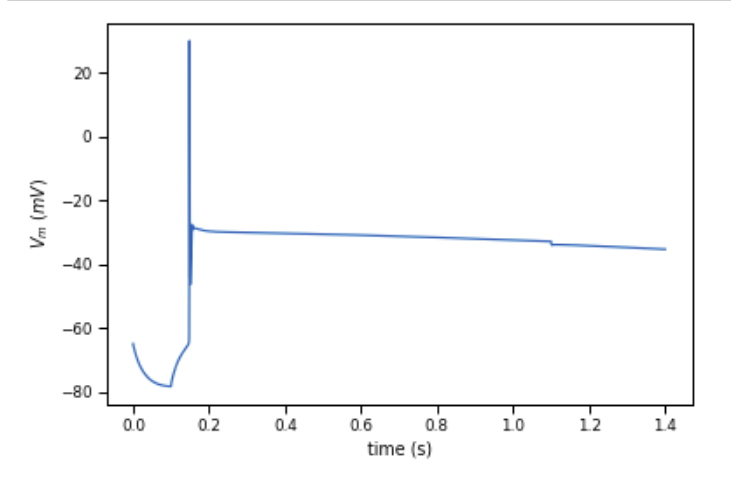
\includegraphics[scale=0.8]{figures/correct_active_l5pc.png}
    \caption[Short duration spike in the L5PC model]{A current injection sufficient for causing a single spike is applied to cell soma, for a whole second from $100ms-1100ms$ in this model. The spike shape is brief and more complicated than reduced model spike shapes. After the very brief spike soma voltage seems to plateau over the entire length of the simulation. The simulation is not long enough for the soma voltage to return to resting membrane potential}
  \label{fig:sub1}
\end{figure}

\begin{figure}
 \begin{center}
    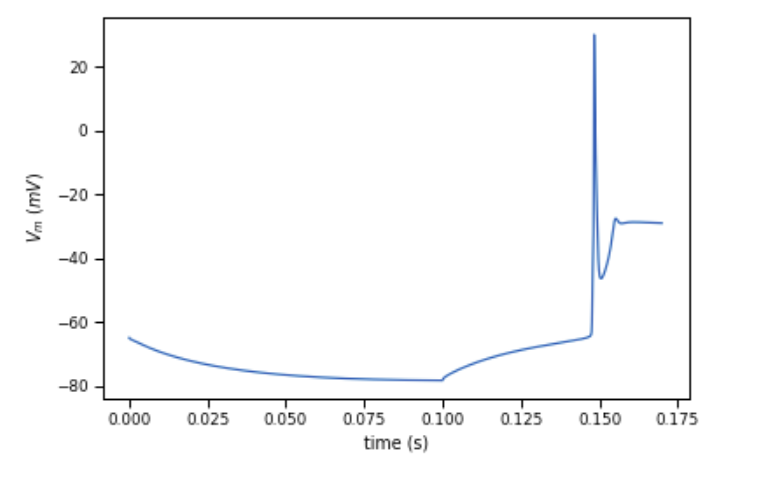
\includegraphics[scale=0.8]{figures/spike_shape.png}
    \caption[Complex spike in the L5PC model]{The above plot warranted a closer look, therefore, this plot features the same model and the same virtual experiment as above, only a smaller time interval has been inflated to fill the whole time axis. In this plot of increased time resolution there is a visible detour in the spikes path to re-polarisation. This unusual feature may be related to a back-propogating dendritic spike, which, a depolarisation wave may have returned from the distal dendrite and has re-invaded the soma, causing the voltage to plateau far above resting membrane potential. These are behaviors, that are obviously neglected in reduced model design}
  \label{fig:sub1}
  \end{center}
\end{figure}

\begin{figure}
\begin{center}
    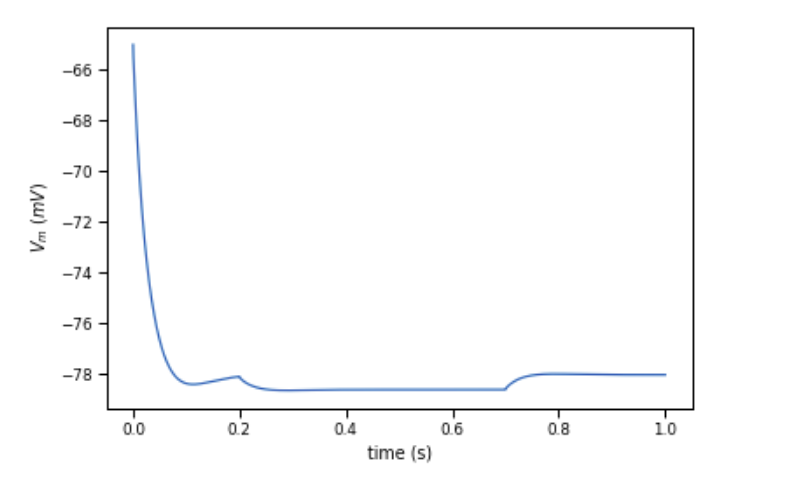
\includegraphics[scale=0.8]{figures/correct_passive_l5pc.png}
    \caption[passive virtual experiment in the Layer 5 Pyramidal Cell]{A current injection value of -$10pA$ is applied to the soma of the pyramidal cell for the duration of $200ms-700ms$. This plot shows the membrane potential at the soma of the multi-compartment model displaying overall expected behavior, the trough of the negative voltage deflection is not as deep as that seen in many reduced models. This suggests the small amplitude of the negative deflection suggests that the L5 PC model is has less resistance than most of the reduced models fitted to the same data, and indeed a low resistance measurement is confirmed in the table below.}
  \label{fig:sub2}
\end{center}
\end{figure}


\begin{table}[ht]
\centering
\resizebox{\textwidth}{!}{
\begin{tabular}{lllll}
\toprule
{} & observations &   predictions & Z-Scores & SEM \\
\midrule
RheobaseTest                   &    213.9 pA &      225.0 pA &  0.065 & 128.9 \\
InputResistanceTest            &  120.7 Mohm &  50.7 Mohm &  -0.90 & 27.9 \\
TimeConstantTest               &     15.7 ms &      16.76 ms &   0.14 & 2.6 \\
CapacitanceTest                &    150.6 pF &     330.7 pF &    1.28 & 1.49 \\
RestingPotentialTest           &    -68.3 mV &     -78.1 mV &   -1.5 & 44.0 \\
InjectedCurrentAPWidthTest     &      1.21 ms &       0.15 ms &   -1.98 & 0.175\\
InjectedCurrentAPAmplitudeTest &     80.4 mV &      89.6 mV &   0.72 & 1.49\\
InjectedCurrentAPThresholdTest &    -42.7 mV &     -59.6 mV &   -2.09 & 1.92\\
\bottomrule
\end{tabular}}
\caption[Z-scores, Observed and predicted features for The Layer 5 Pyramidal Cell]{As the Layer 5 pyramidal cell was made eligible for neuronunit testing. A suite of relevant Neuroelectro L5 Pyramidal cell tests were applied to this cell model iterative in an optimization framework. This table shows the end result of this process, where agreement between model and experiment has been maximized. The result of the test shows that the model falls within the range of biological plausibility, although model results are far from perfect in all tests. Notably the Rheobase value agrees well with experiments, as does the membrane time constant}
\end{table}


%\caption[Observed and Predicted L5PC]{Observations, predictions, and Z-scores pertaining to the NeuronUnit-optimized Layer 5 Pyramidal Neuron}
\label{tab:l5pc_table}
The corresponding statistics were
$(\chi^{2},p_{value})=(13.56, 0.094)$.
Note that the p-value is not sufficiently low to reject the null hypothesis that this model neuron is not from the same distribution as the biological/experimental results.
This may reflect the highly variable nature of the biological/experimental results, rather than the verisimilitude of the optimized model.
Nonetheless, given this experimental variability, the optimization is at least satisfactory. It is also worth noting that not all optimization results lead to the same solution, between different model fitting routines, the optimizer had to choose between fitting the membrane time, constant, fitting the spike width, and fitting the input resistance as the model could be made to fit only one of these measurements at a time. In other words in this model: input resistance, time constant, and spike width were conflicted.

%Hind-limb
%\cite{van2016bluepyopt}
%To understand the validity of model re-purposing, we tested a model constrained on Layer 5 Somatosensory cortex Pyramidal neurons. 

There were two points to this exercise: the first point was to show that multi-compartment conductance based models, are very slow to evaluate, and the second point was, that without enough time, the results are not necessarily as good as you would expect for the inclusion of additional complex mechanisms. There is an unintended straw man character to this observation, it's stipulated in the model documentation (a python notebook) that the model would require a run of at least $100$ generations and a population size of $100$ too properly optimize relative to a different set of constraints. Unfortunately I did not have the time or the computer resources to apply the specified optimization job. However these time considerations bolster a different assertion from my thesis work, timeliness of simulation results aids model refinement, whereby brief simulation times improves scientific insight.
However, the model itself happens to be a determining factor in reducing time. The resulting optimized model might serve as a useful benchmark, for us to evaluate the relative performance of reduced model fits. 

A suite of Neuronunit tests containing the tests: rheobase value, membrane voltage time constant ($\tau_{m}$), input resistance was computed. 
% somatosensory cortex, or cell from the l5 somatosensory rat, hind leg region, so it is probably not comparable to NeuroElectro Data.

Significant development work went into making the model eligible to take NeuronUnit tests, and amenable to NeuronUnit driven optimization, to make this complicated conductance based multi-compartment model interoperable with the NeuronUnit test judging paradigm.
The intention is that by making this model inter-operable with NeuronUnit the model will be able to amenable to different, optimization. 

%\begin{figure}
%    \begin{center}
%    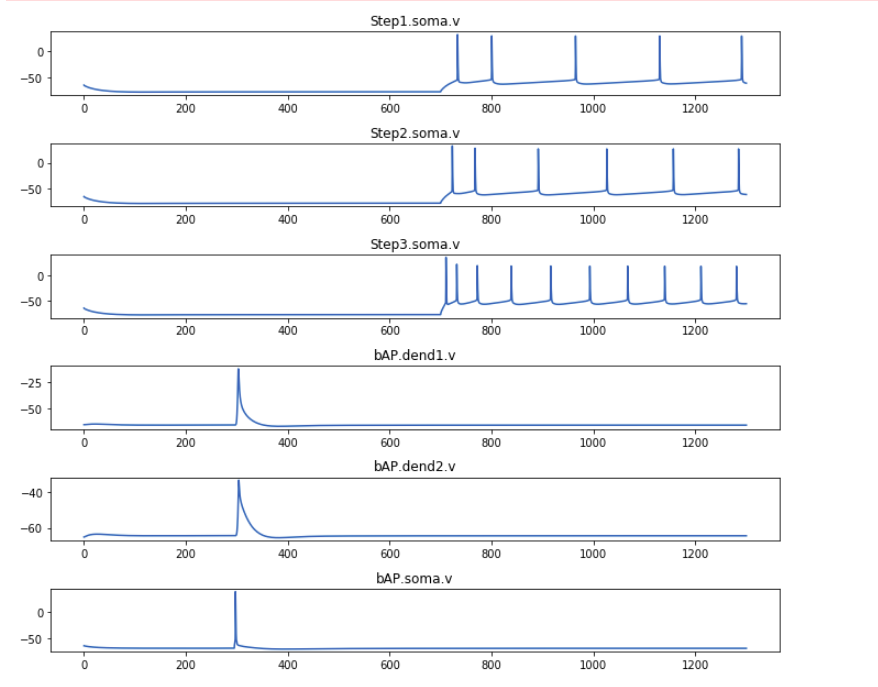
\includegraphics{figures/l5pc_before_opt}
    % \label{fig:my_label}
%    \end{center}
%\end{figure}


%Behavior of the L5PC model is explored under three different stimulus strengths.

\begin{figure}
    \begin{center}
    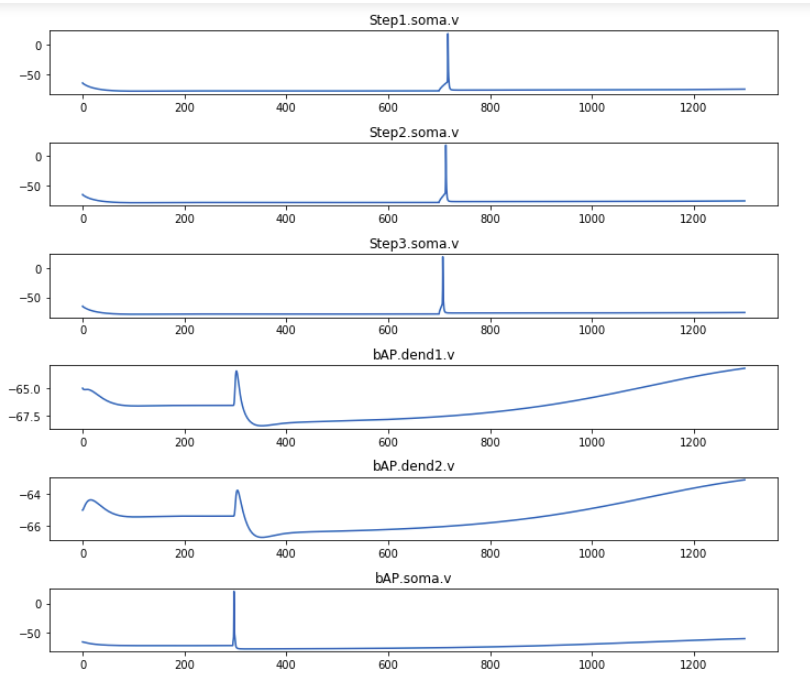
\includegraphics{figures/l5pc}
    \caption[Behavior of the L5PC model under optimized parameters]{Behavior of the L5PC model is explored under only one stimulus strength. Membrane potential this time is viewed from recording locations in the soma and dendrites.  Membrane potential this time is viewed from recording locations in the soma and dendrites. In this recording site at the dendrite there is a singular backpropogating spike. Although the soma and axon hillock, trigger an adapting spike train, lasting more than a second, the dendrite only receives one backpropogating potential, which has a large spike half width. The reason the axon fires multiple times, but the dendrites fire once, is because  dendrites contain dominating passive mechanisms, that can low pass filter invading currents} 
    \label{fig:after_optimization}
    \end{center}
\end{figure}    
    %\caption[Behavior of the L5PC model before optimization under default parameters]{}
%   }


\begin{figure}
    \begin{center}
    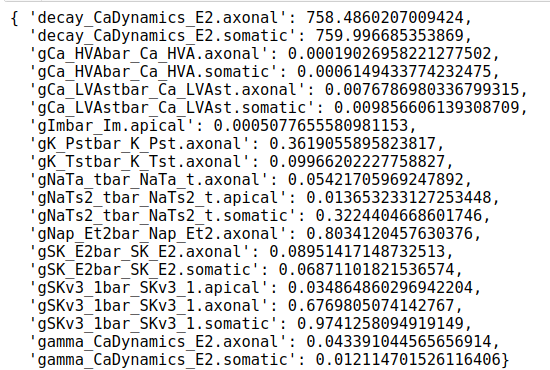
\includegraphics{figures/parameters_opt_l5pc.png}
    \caption[Subset of modal parameters eligible for tuning in L5PC neuron]{Here I list not all the parameters of the layer 5 model, just the subset of adjustable parameters. The parameters that the genetic algorithm modifies, they are listed here with their default values. There are 20 different parameters that two different locations in the neuronal tree. The fact that there are 20 different dimensions to optimize over makes this problem especially intractible for the average researcher, since it is slow to evaluate as well as high dimensional. With the exception of the GLIF model, most models considered here are $<14$ parameters.}
    \label{fig:ca1_parameters}
    \end{center}
\end{figure}


%\begin{figure}
%\begin{center}
%   \includegraphics[scale=0.8]{figures/correct_a%ctive_l5pc.png}
%    \caption{A current injection sufficient for %causing a single spike is applied for a whole %second from $100ms-1100ms$}
%  \label{fig:sub1}
%  \end{center}
%\end{figure}

%As a reference point for understanding 
%    \caption{The spike shape is very brief in duration, and so it is worth zooming in for a closer look}

%\begin{figure}%{.2\textwidth}
%  \begin{center}
%    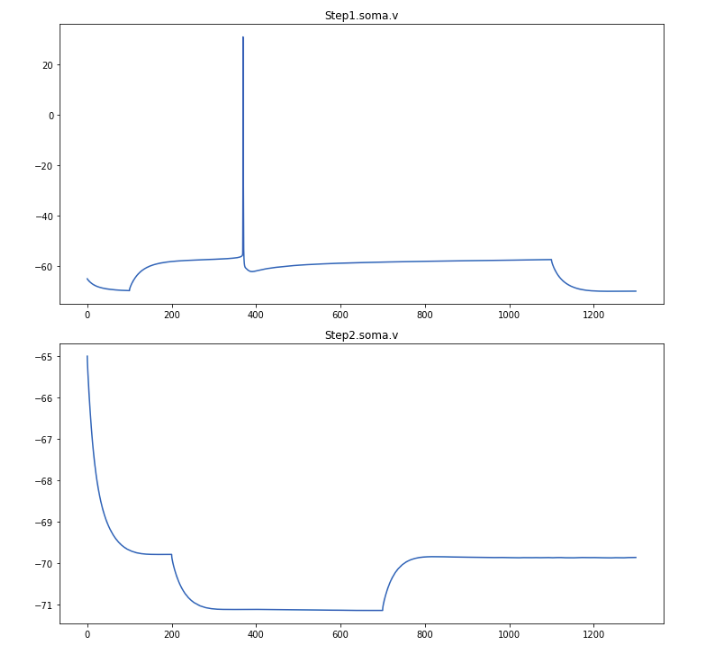
\includegraphics[scale=0.8]{figures/L5Somatosensory_not_optimized.png}
%    \caption[Plot of at threshold firing pyramidal neuron]{$V_{m}$ in $(mV)$ versus time $ms$, plots include a above threshold (top) and below threshold stimulus (below)}
%  \label{fig:brief_shape}
%  \end{center}
%\end{figure}

%\begin{figure}%{.2\textwidth}
%  \begin{center}
%    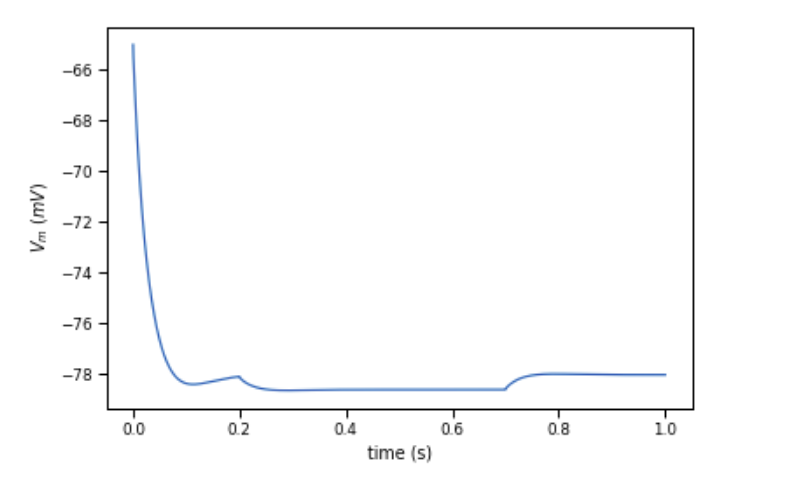
\includegraphics[scale=0.8]{figures/correct_passive_l5pc.png}
%    \caption[plot of negative amplitude current stimulus]{A current injection value of -$10pA$ is applied to the cell for the duration of $200ms-700ms$}
%  \label{fig:passive_properties}
%  \end{center}
%\end{figure}


A test suite was constructed using NeuroElectro for the non specific [cortical regions] layer 4/5 cortex pyramidal cell, and we were able to evaluate this layer 5 PC cells against the criteria of the neuroelectro test suite. Note the unnatural looking brief spike duration of the model cell spike  \ref{fig:brief_shape}. It is possible that the majority neuroelectro experiments on the layer 5 pyramidal cell were conducted under room temperature as opposed to body temperature, as there is evidence that the temperature of cortical tissue modulates spike width \cite{goldin2017temperature}, in particular cooling can contract their spike width

%%
% https://neuroelectro.org/data_table/36261/
%%
% from spike width table: 0.65 ± 0.13	1.04 ± 0.25**	0.51 ± 0.03**	0.59 ± 0.06	0.61 ± 0.03
%%
%


Due to computational limitations this model was only run for 
$12$ offspring, and $30$ generation. Actually a minimum of $\mu=100$, $NGEN =100$ was prescribed by the scientists who optimized the initial model, however such a large compute job required prohibitive computational resources.

The unoptimized model had statistics:
$(\chi^{2},p_{value})=(13.56, 0.094)$

The optimized model produced statistics
$(\chi^{2},p_{value})=(6.63, 0.57)$

Optimization then clearly improves the model, however, it does not bring the model  biological plausibity.
This can be improved by omitting some of the worst tests, overall, the tests are compromized.



It is worth noting that the layer 5 neocortical pyramidal neuron was very slow to dispatch relative to the reduced models developed in this thesis work. Where as a typical reduced model described here evaluated in the order of $~0.0025 seconds$, this model on average took $5.74$, for a single run and $34.8$ to solve for the models Rheobase, current.

This model was pre-optimized to fit to spike times and F/I mainly, and so it should not necassarily be expected to fit other electrical charactersistics of the cell. Only the rheobase test, and the time constant test seemed to fall within the range of biological plausibility.
None the less, this model remains a useful benchmark for reduced neuronal models. 
\subsection{Gallery of Model Fits to Supra-threshold Experiments}
\begin{comment}
\begin{figure}
    \centering
    \begin{subfigure}[t]
        \centering
        \includegraphics[width=0.5\linewidth]{example-image-a.pdf} 
        \caption{Generic} \label{fig:timing1}
    \end{subfigure}
    \hfill
    \begin{subfigure}[t]
        \centering
        \includegraphics[width=0.5\linewidth]{example-image-b.pdf} 
        \caption{Competitors} \label{fig:timing2}
    \end{subfigure}

    \vspace{1cm}
    \begin{subfigure}[t]
        \centering
        \includegraphics[width=0.5\linewidth]{example-image-c.pdf} 
        \caption{Price regulation} \label{fig:timing3}
    \end{subfigure}
    \hfill
    %\begin{subfigure}[t]%{0.45\textwidth}
    %    % just an empty subfigure to shift C below A
    %\end{subfigure}
    \caption{Some general caption of all the figures. In (\subref{fig:timing1}) you can see a  green square....}
\end{figure}
\end{comment}

% TODO make multi panel.

\begin{figure}
    \centering
    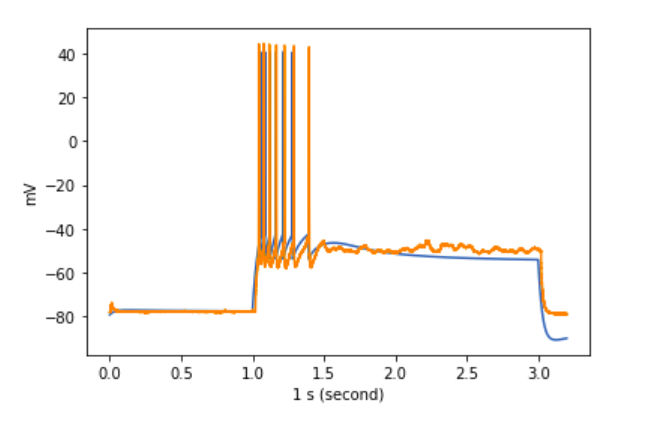
\includegraphics[scale=0.75]{figures/adexp_fit_allen_spec_id_476053392.png}
    \caption{An adaptive Exponential Model was fitted to both the spike time, and spike shape data in a sweep from Allen specimin id: 476053392} \label{fig:specimen_476053392}
\end{figure}

\begin{figure}
    \centering
    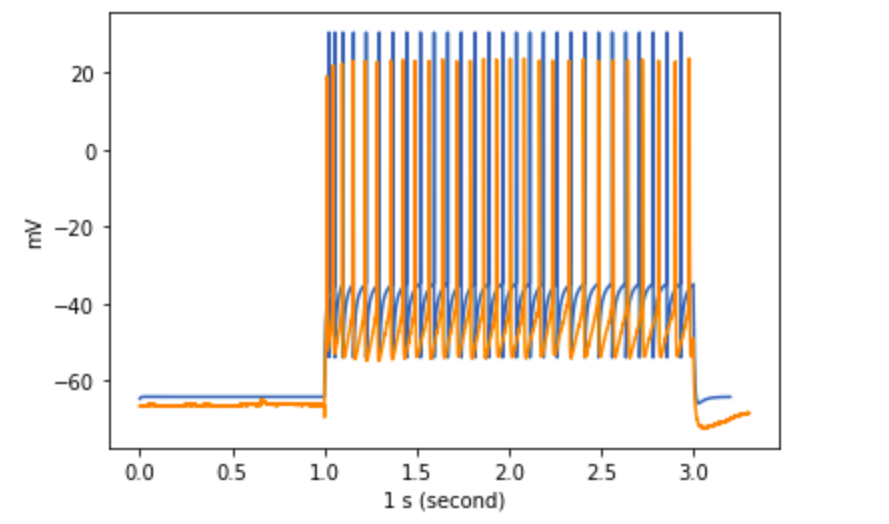
\includegraphics[scale=0.75]{figures/28spikesB95}
    \caption{An adaptive Exponential Model was fitted to both the spike time, and spike shape data in a sweep from Allen specimin id: 476053392} \label{fig:specimen_476053392}
\end{figure}

%Similar to Druckmann Suprathreshold depolarizing step currents \cite{druckmann2008evaluating}.
\begin{figure}
    \centering
    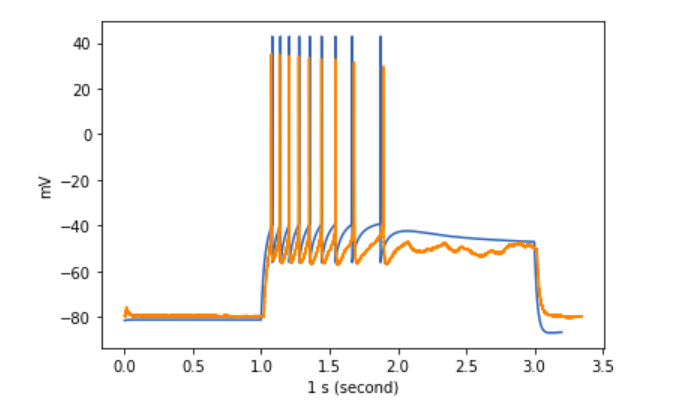
\includegraphics[scale=0.75]{figures/adexp_fit_allen_specid_325479788.png}
    \caption{ An adaptive Exponential Model was fitted to both the spike time, and spike shape data in a sweep from Allen specimin id: 325479788}
    \label{fig:specimen_325479788}
\end{figure}


% Interesting direct qoute from Druckmann:
%"In experiments, intrinsic noise gives rise to a large variability (e.g., in firing pattern) in the voltage responses to repetitions of the exact same input. Thus, the common approach of fitting models by attempting to perfectly replicate, point by point, a single chosen trace out of the spectrum of variable responses does not seem to do justice to the data."

%In experiments, however, when the exactly same stimulus is repeated several times, the voltage traces elicited differ among themselves to a significant degree (Mainen and Sejnowski, 1995; Nowak et al., 1997).

A joint collection of current injections and recordings known as sweeps were taken from a rat somato-sensory hind limb neuron.
\ref{fig:B95Adexp} is a challenging waveform to fit, as adaption does not predict the final ISI, which is smaller than the penultimate one. 

Although it is not obvious there is significant variation in ISIs (although the range of that variation may be concentrated within a small margin). As noted in the literature \cite{druckmann2007novel} it is probably mis-founded to over fit models to exact spike times because neurons themselves experience noisy intrinsic currents and they are likely to illicit different spike trains, given identical presentation of stimulus. In hind-sight I propose, to optimize on FI-slope and spike rate, while comprimizing on exact spike time agreement.

\begin{figure}
    \centering
    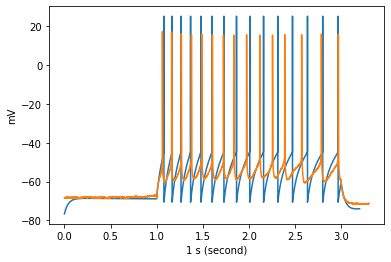
\includegraphics[scale=0.75]{figures/bbp_multispiking_fit.png}
    \caption{An adaptive Exponential Model was fitted to both the spike time, and spike shape data in a sweep from animal B95 
    %\url{http://microcircuits.epfl.ch/#/animal/8ecde7d1-b2d2-11e4-b949-6003088da632}
    Blue Brain Project. The base voltage. The base voltage, and Resting Membrane Potential, and spike numbers are matched, spike times are not perfectly aligned, spike height, and trough depth are not perfectly matched}
    \label{fig:B95Adexp}
\end{figure}

\begin{figure}
    \centering
    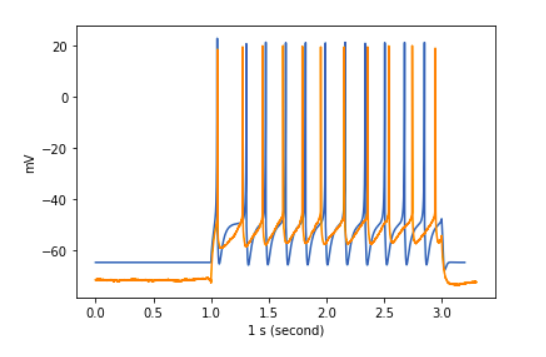
\includegraphics{figures/IZHI_B95.png}
    \caption{An Izhikevich model was fitted to both the spike time, and spike shape data in a sweep from Blue Brain Project. The Spike amplitude, and spike numbers are matched, spike times are not perfectly aligned}
    \label{fig:B95_IZHI}
\end{figure}

In figures \ref{fig:B95Adexp}, you can see that although several aspects of the waveform are fitted, exact spike times are not always fitted \ref{fig:B95_IZHI}

The result that the adaptive exponential model is better able to fit spike times than the Izhikevich model is consistent with the literature \cite{rossant2011fitting}. the figure below shows results from the INCF modelling competition the adaptive exponential model and families of models related to it such as the MAT model (made to order Multiscale Adaptive Time window) model, are significantly better able to fit to spike times than the Izhikevich model.



\begin{figure}
    \centering
    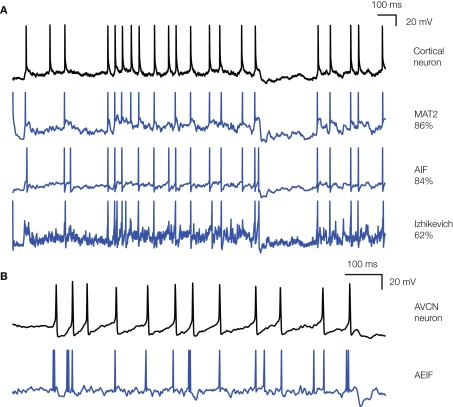
\includegraphics[scale=5.0]{figures/IZHIkevich_fit_60Adexp_80.jpg}
    \caption[The spectrum of model fits]{This great figure from the publication: \citep{rossant2011fitting} shows how the majority of models that fit spike time, do not also fit spike shape. Spike shape and AP timing constitute a persistent conflicted priority with regards to model fitting. Included in this figure are fits from reduced models used in this work AIF, and Izhikevich model.
    }
    \label{fig:my_label}
\end{figure}

%3. Study of variance between models and data.  The optimized models part of this section is predicated on result 1b (so that optimization results can be believed).  You already have the poster for this.
%I think this captures most of your results in three themes.  Other results which are really methods, like parallel rheobase search, can stay in the methods, and you will get credit for them there.

\section{Published models vs optimized models}

It is known that neural models and experimental measurements generally diverge in important ways, however, it is desirable to know the specific sources of divergence. Models and experiments may disagree for two reasons: \emph{A} the model is not flexible enough to satisfy a particular constraint simultaneously to a collection of constraints, or, \emph{B} the model was incorrectly fitted to the a type of conflicting constraints (for example model fitted to spike times at the expense of Rheobase, and FISlope). 

Since we don't yet have complete knowledge of model/experiment divergence, we don't necessarily know the best features to target with regards to model fitting. Specific knowledge of model/data disagreement facilitates the prioritized selection of features that should guide optimization. 

%\begin{figure}
%    \centering
%    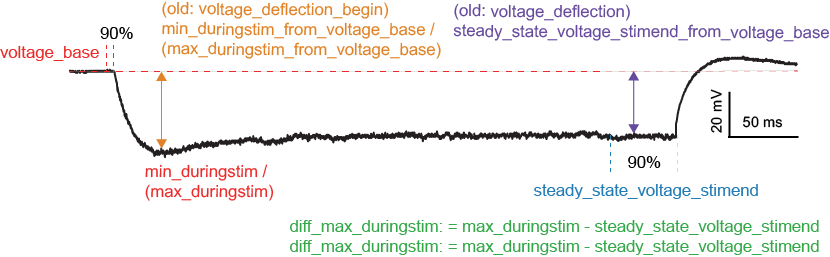
\includegraphics{figures/voltage_features.png}
%    \caption{Caption}
%    \label{fig:voltage_figures}
%\end{figure}
%\begin{figure}
%    \centering
%    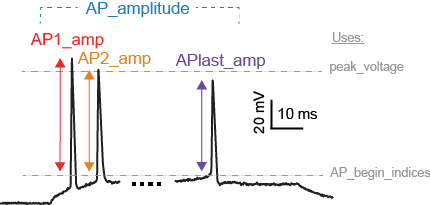
\includegraphics{figures/AP_Amplitude.png}
%    \caption{Caption}
%    \label{fig:features_example}
%\end{figure}

%\begin{figure}
%    \centering
%    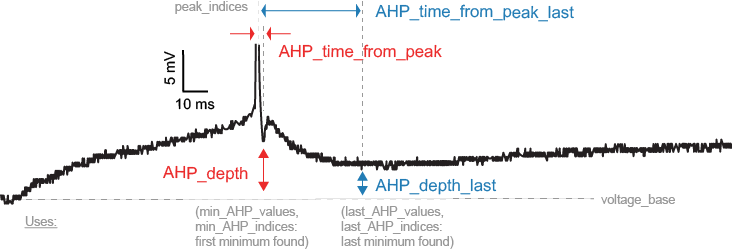
\includegraphics{figures/AHP.png}
%    \caption{After hyperpolarisation potential }
%    \label{fig:features_example_ahp}
%\end{figure}


%\begin{figure}
%    \centering
%    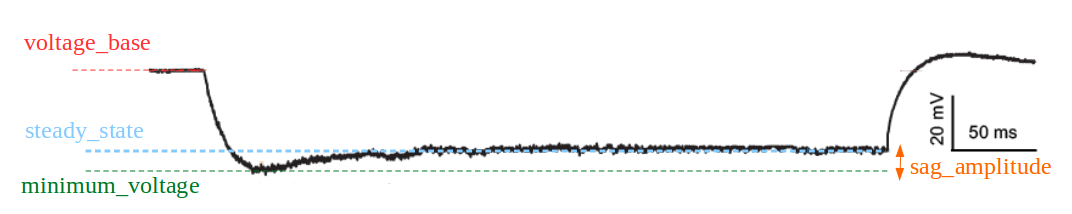
\includegraphics{figures/sag_amplitude}
%    \caption{Caption}
%    \label{fig:sag_amplitude}
%\end{figure}


\subsection{Features} 

For many of these features it will be useful to refer back to the methods \ref{sec:data_sources} section, where I some key features were depicted. 

Consider a voltage recording at the location of the membrane of a neuron. Teams of researchers have already segmented voltage recordings into labelled sections, each section has a classification that is based on the shape of waveform in a limited region see figure \ref{fig:voltage_figures} for example. Rather than specifying by name each measurement it is often useful to refer collectively to these measurable shapes as "features". 

In the following multivariate analysis we analyze hundreds of such features, and we summarize important differences in a subset of this high dimensional feature space.  Below, I describe some neuronal model features that agreed well with experiments, and some features that diverged.


\subsection{Publications Associated with Model Sources}
$972$ models, $448$ experiments.
$1276$ samples. This did not include some blue brain cells. After data cleaning many data points were dropped.  $244$
$1420$


Allen Institute for Brain Science Cell Types Database [7] can be accessed using the SDK.  The Blue Brain Project Dataset can be obtained from the Data Navigator, or an API.

\begin{itemize}
\item Allen Institute V1 \cite{gouwens2018systematic}
\item Somatosensory Cortex \cite{markram2015} 
\end{itemize}

\subsubsection{Feature Extraction Libraries}
\begin{table}
\centering
%\resizebox{\textwidth}{!}{
\begin{tabular}{lll}
%\toprule
{} EFEL Ephys Feature Extraction Library & AllenSDK & Druckmann (2012) 
%\bottomrule
\end{tabular}
%}
\end{table}




\begin{tabular}{lll}
%\toprule
{} Injection 1 & Injection 2 & Injection 3 \\
 at $1.0 \times$ Rheobase & at $1.5 \times$ Rheobase & at $3.0 \times$ Rheobase 
%\bottomrule
\end{tabular}




%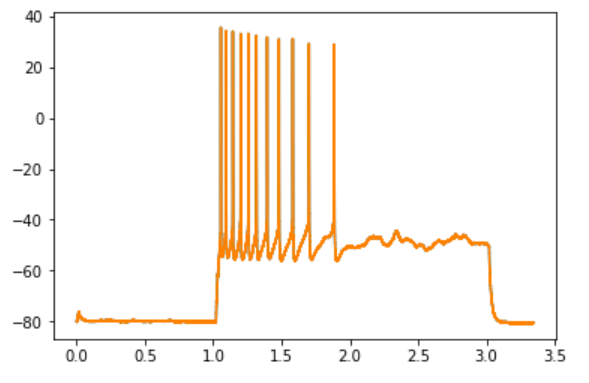
\includegraphics[]{chapters/app_tex/Allen_rush}
\begin{figure}
    \begin{center}
    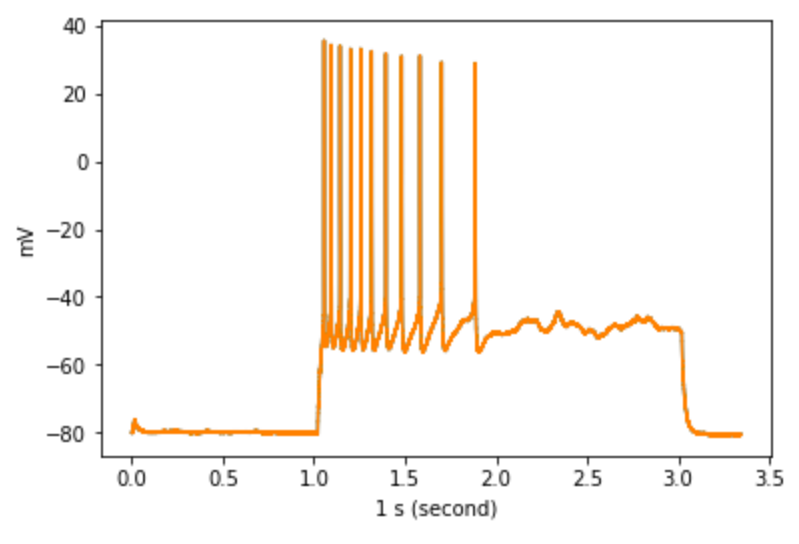
\includegraphics[width=0.6\linewidth]{figures/multi_spiking_large_allen}
    \caption{A voltage recording from a supra-threshold experiment waveform used as a basis for the Allen Brain Institute cell types data base. Publication Gouwens rat \cite{gouwens2018systematic}}
    \label{fig:adaptionm}
    \end{center}
\end{figure}    

\begin{figure}  
    \begin{center}
    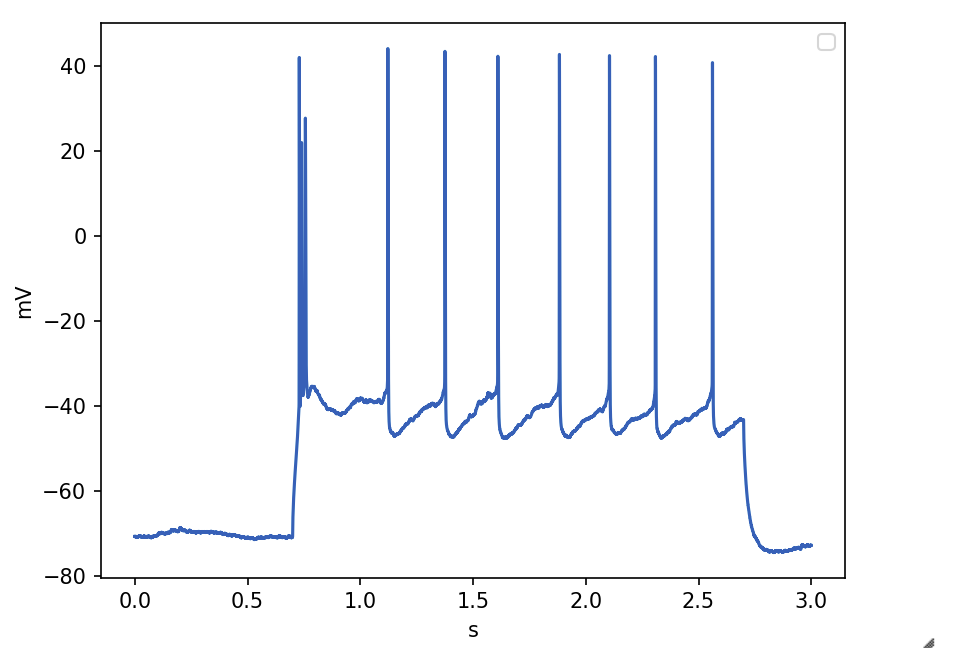
\includegraphics[width=0.6\linewidth]{figures/multi_spiking_large_bbp}
    \caption{Another example of a supra threshold experimental protocol. Publication Jouvanile rat \cite{toledo}}
    \label{fig:bbp_trace_adaption_late_spike}
    \end{center}
\end{figure}    

In order to identify electrical measurements or "features" that were responsible for the most variance in models and in-vitro, we performed Sparse Principle Component Analysis \cite{zou2006sparse} on the combined pool of model and in vitro experiments. 



\subsection{sources of disagreement}

The key advantage of using sparse PCA is the results are readily interpret able. A common sceanario in regular Principal Component Analysis is you may obtain a low dimensional embedding plot made from unit rotation vectors that maximize variance, but no way of relating the reduced dimensions back to the sources of variance in the system of interest. 

Sparse PCA yields an interpretable list of features, that build the principle components. This list of features is ranked and sorted with respect to their total contributions to the Eigen Vectors. Since two Eigen Vectors where made these are.

Principle component 1 had non zero loadings for ranked (highest to lowest).
The first Eigen Vector does not facilitate discrimination between models and experiments, but the second Eigen Vector spaces models and experiments into three seperate clusters.
\begin{verbatim}
upstroke_t_1.5x allen 
peak_t_1.5x allen 
threshold_t_1.5x allen 
fast_trough_t_1.5x allen 
fast_trough_t_3.0x allen 
upstroke_t_3.0x allen 
peak_t_3.0x allen 
threshold_t_3.0x allen 
peak_indices_1.5x efel 
min_AHP_indices_1.5x efel 
\end{verbatim}

Principle component 2 had non zero loadings for ranked (highest to lowest)
\begin{verbatim}
fast_trough_index_1.5x allen 
peak_index_1.5x allen 
upstroke_index_1.5x allen 
threshold_index_1.5x allen 
fast_trough_index_3.0x allen 
peak_index_3.0x allen 
upstroke_index_3.0x allen 
threshold_index_3.0x allen
\end{verbatim}

These are the weighted features that were used to make Eigen vectors 1 and 2, are responsible for most of the variance. Interestingly these features mostly belong to the Allen SDK feature extraction set, with two exceptions: $peak_indices_1.5x$ $min_AHP_indices_1.5 \times$ belonging to EFEL efel 

%Move to Discussion 
Another observation is that a small majority of features used to create the sparse Eigen Vectors, are in the range of $1.5$ * rheobase, and slightly fewer are features from a $3.0\times$ rheobase experiment. A reason for this is as follows, larger spike time variability $C_{V}$ is expressed in intermediate ranges of current injection. Under the highest current injections, high frequency evenly spaced spikes are likely, although spike frequency adaption is possible, the higher current may force to spikes to occur promptly after their refractory period, and in this case you might observe diminishing amplitude of spikes with increasing stimulus duration.

At $1.5 \times rheobase $ I believe there to be more spike time variation, at $3.0 \times rheobase $  I believe there to be more spike amplitude variation.

\subsection{Sparse PCA}
Sparse PCA revealed five overlapping different groups of neuronal identity's, and three non overlapping clusters. Models and experiments clustered separately to each other in the low dimensional space. Models and data were easily separable in the direction of the 2nd Eigen Vector.

%The first principle component 
Models and experiments shared the same breadth of variability across the first principal component, with only slightly more variance in the experiments than in the data. Allen cell types experiments seemed to encompass the most variability out of models and experiments across all data sets. Models clustered tightly and varied less than in vitro experiments.



Although imputation was successfully used to avoid dropping a large number of samples, about half of all initial BBP/Allen models data types were excluded from a final analysis, because they did not all capable of meeting inclusion criteria.  

\ref{fig:reference_feature_list}
List of complete 47 features used in the analysis down from 466 after data cleaning.


There was one group of Allen cell type experiments that clustered on their own, making one set of the cluster.

sparse PCA 2nd Eigen Vector. 
Disagreement between models and in-vivo neurons may reflect limitations of model design and can be investigated by probing the key features used by classifiers to distinguish these two populations. 

\begin{figure}    
\begin{center} 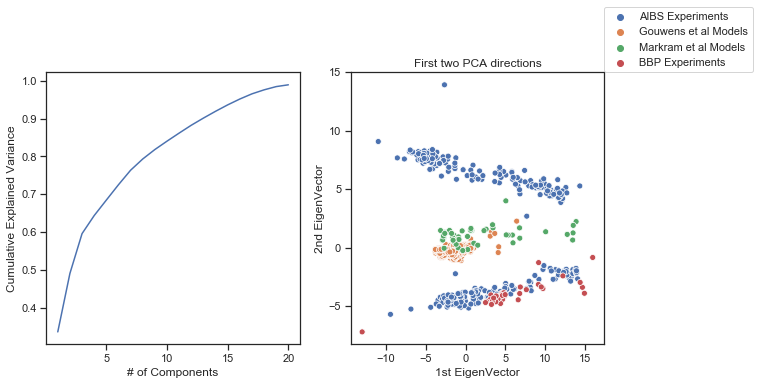
\includegraphics[width=1.0\linewidth]{figures/cortical_model_data_agreement_52_1}
    \caption{}
    \label{fig:}
\end{center}
\end{figure}    
\begin{figure}    
    \begin{center}
    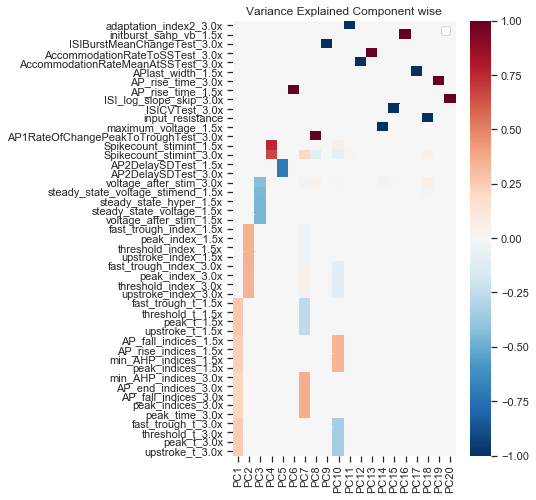
\includegraphics[width=1.0\linewidth]{figures/cortical_model_data_agreement_54_1.png}
    \caption{}
    \end{center}
\end{figure}    
\cite{wang2019sag}

\begin{figure}
    \centering
    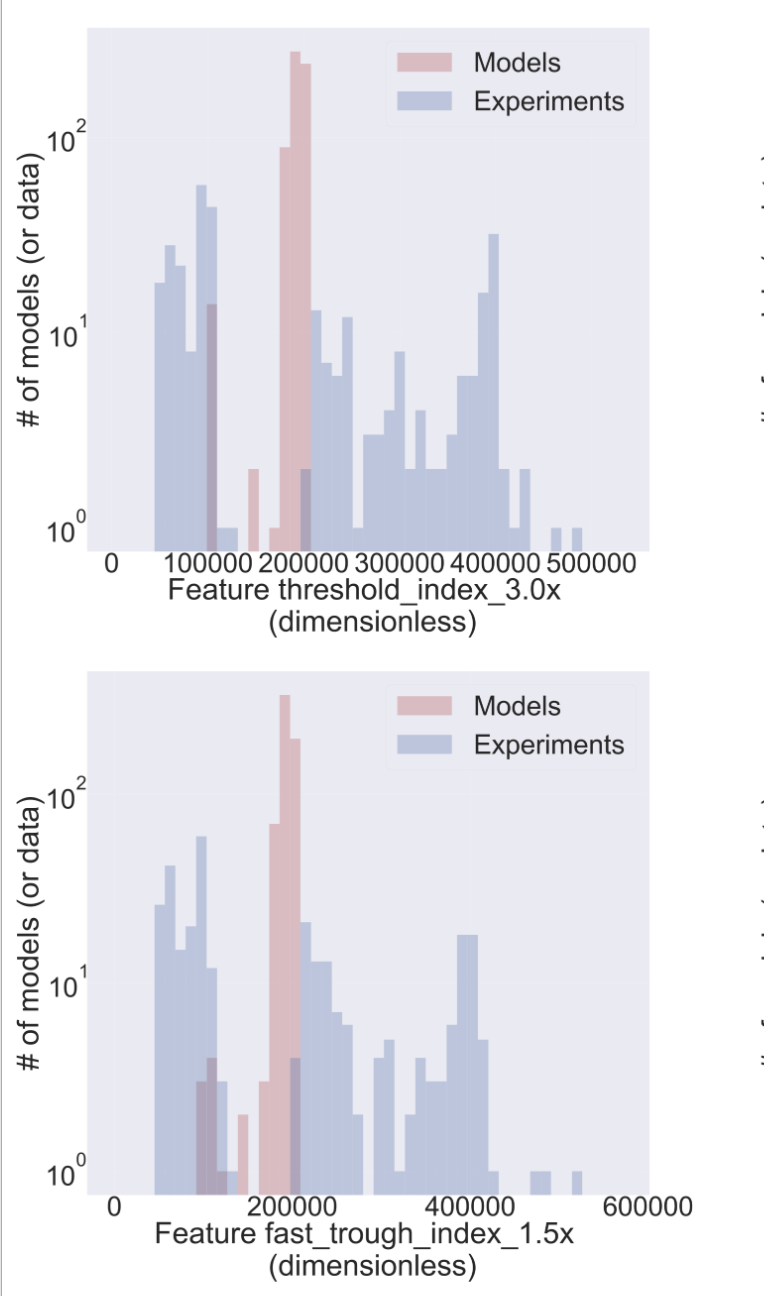
\includegraphics{figures/features_that_disagree}
    \caption{Caption}
    \label{fig:from_poster_disagree}
\end{figure}




\begin{itemize}
    \item upstroke\_t\_1.5x allen feature
    \item  peak\_t\_1.5x allen feature
    \item threshold\_t\_1.5x allen feature
    \item fast\_trough\_t\_1.5x allen feature
    \item fast\_trough\_t\_3.0x allen feature
    \item upstroke\_t\_3.0x allen feature
    \item peak\_t\_3.0x allen feature
    \item threshold\_t\_3.0x allen feature
    \item peak\_indices\_1.5x efel feature
    \item min\_AHP\_indices\_1.5x efel feature
\end{itemize}


\begin{itemize}

    \item fast\_trough\_index\_1.5x allen feature
    \item fast\_trough\_index\_3.0x allen feature
    \item threshold\_index\_1.5x allen feature
    \item peak\_index\_1.5x allen feature
    \item upstroke\_index\_1.5x allen feature
    \item peak\_index\_3.0x allen feature
    \item upstroke\_index\_3.0x allen feature
    \item threshold\_index\_3.0x allen feature
\end{itemize}

After identifying specific sources of model and experiment divergence, it is now possible in theory to start fitting models which  seek to resolve specific types of disagreement. However, as alluded to in the introduction, it was found that were two other important factors. 

%Model repurposing is common and it is done on a network scale \cite{traub} and an individual cell scale.
%Experimental evidence is starting to reveal that model re-purposing of pyramidal neurons might not be a good idea.

%Scientific insight is well-served by the discovery and optimization of abstract models that can reproduce experimental findings. NeuroML (NeuroML.org), a model description language for neuroscience, facilitates reproducibility and exchange of such models by providing an implementation-agnostic model description in a modular format. NeuronUnit (neuronunit.scidash.org) evaluates model accuracy by subjecting models to experimental data-driven validation tests, a formalization of the scientific method. 


% After applying dimensionality reduction to this very high dimensional feature space, we show that the real (biological neurons) and simulated (model neurons) recordings are easiley and fully discriminated by eye or any reasonable classifier.  

% Are they still discernable?
%972 models, 448 experiments.


%Consequently, not a single model neuron produced physiological responses that could be confused with a biological neuron. Was this a defect of the model design (e.g. key mechanisms unaccounted for) or of model parameterization? We found that if we introduced models that were revised via optimization the revised models overlapped with the distribution of biological neurons, and were mostly classified as such. 

\section{A Web Application for Optimization and Visualization}
An application was developed using the reduced model neural model optimizer as flexible backend. %Since the optimizer essentially acts like the backend of a program, creating an application simply meant writing a "front-end".\\
\\
A python webframe "streamlit" facilitates the construction of web applications. Fortunately for the developer, coding in this frame work requires no handling of html elements, and streamlit has tools for acting on important high level data structures, such as the pandas data frame, matplotlib graphs and plotly graphs.\\
\begin{figure}
\begin{center}

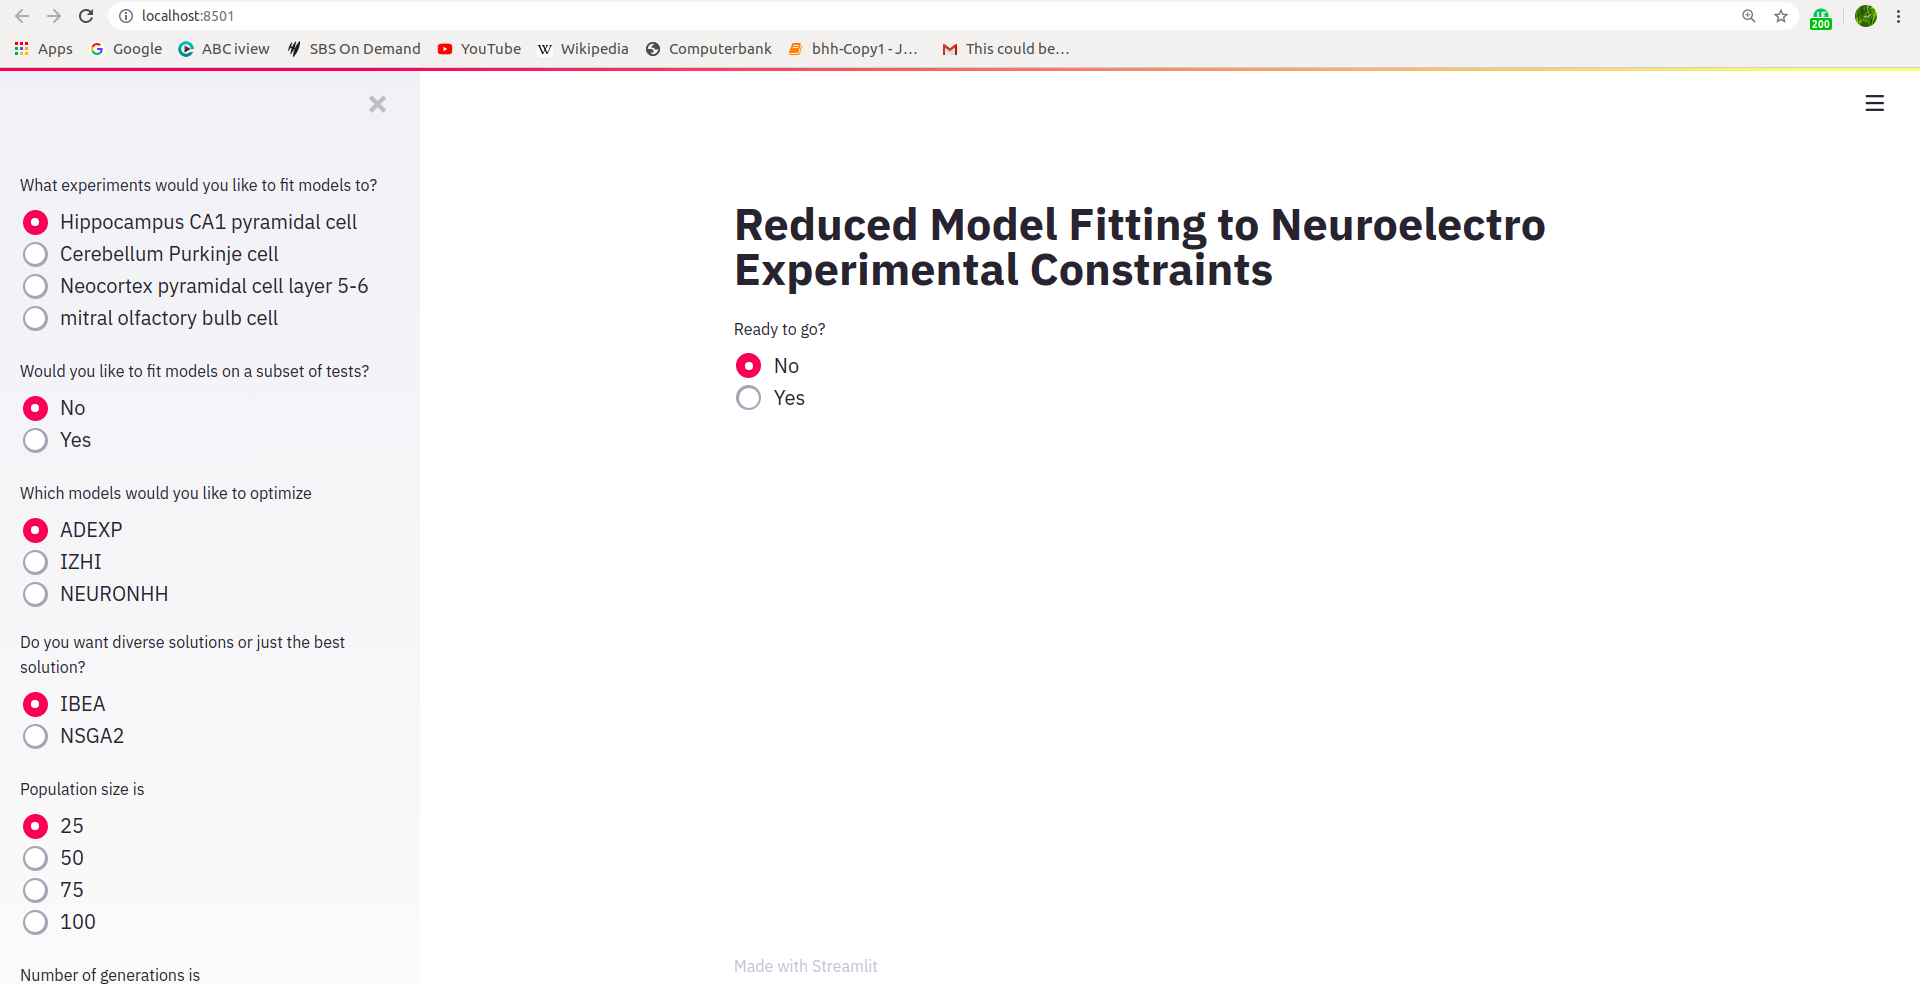
\includegraphics[scale=1]{chapters/app_tex/web_app_thesis}
\caption{The side-pane of the web application provides users with a choice of three models, and four data sets that can be used to fit data.
}
\end{center}

\end{figure}
\begin{figure}
\begin{center}

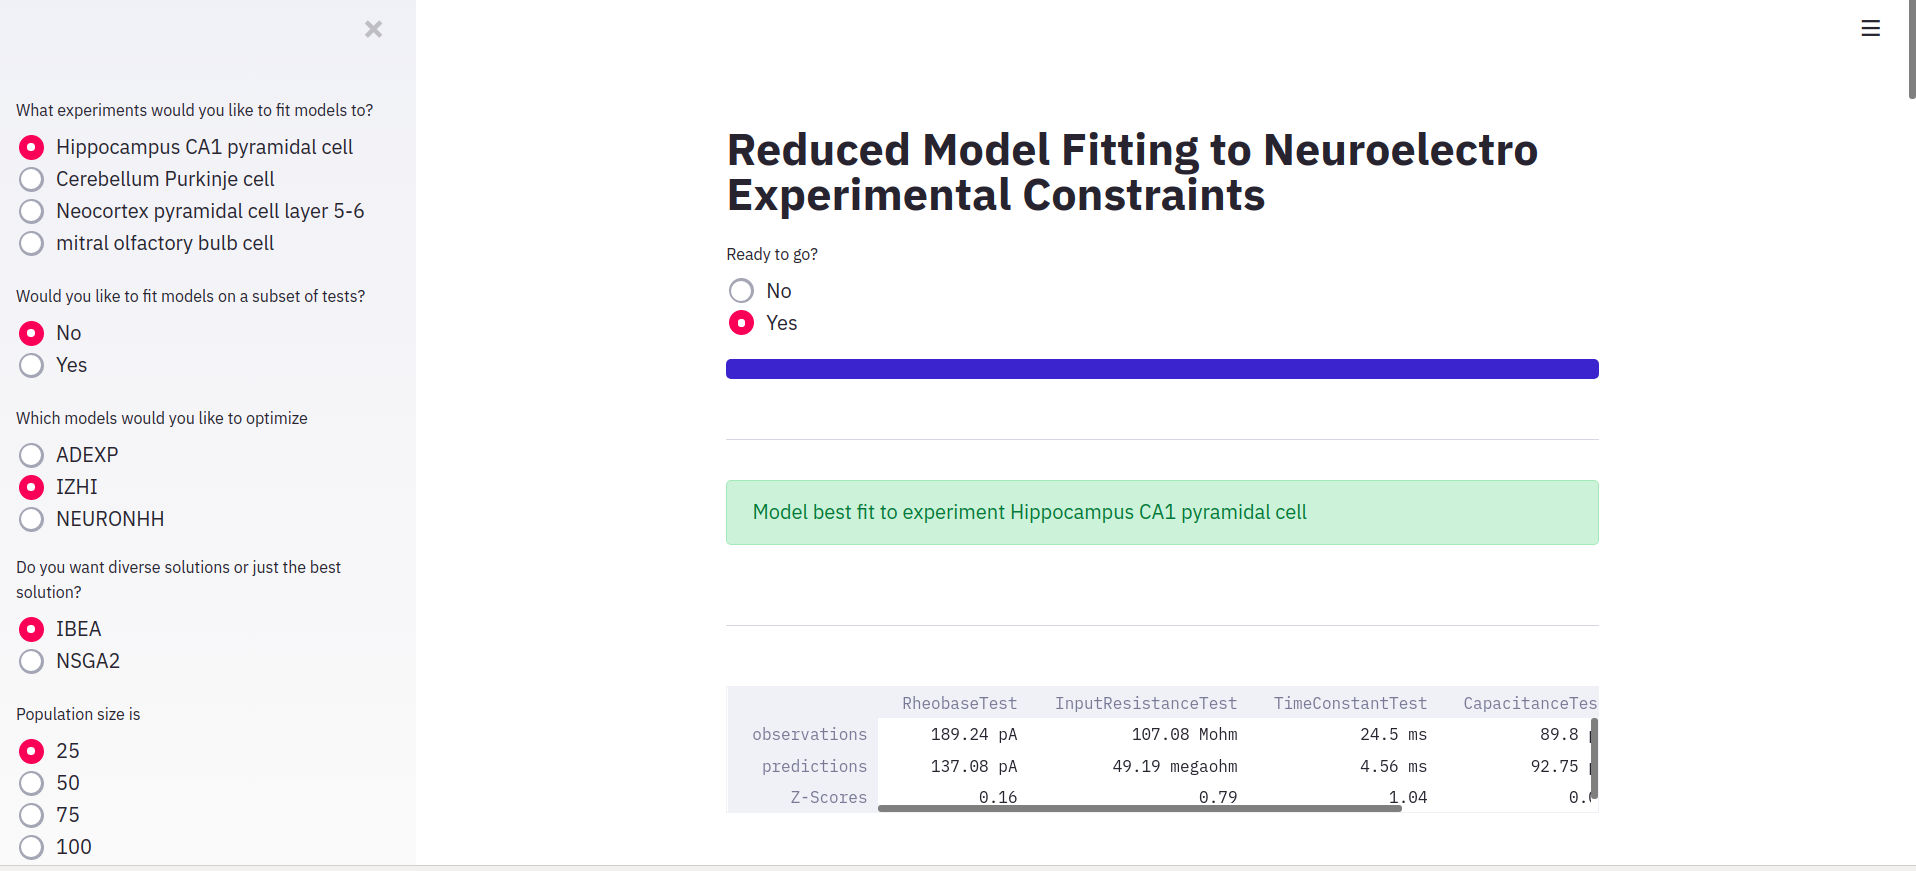
\includegraphics[scale=1]{chapters/app_tex/app_results}
\end{center}

\end{figure}

When optimization is complete, the user sees the $\chi^{2}$ statistic, the $p$-$value$. The user is then allowed to follow a link to download the "model", python object code.\\
\begin{figure}
\begin{center}

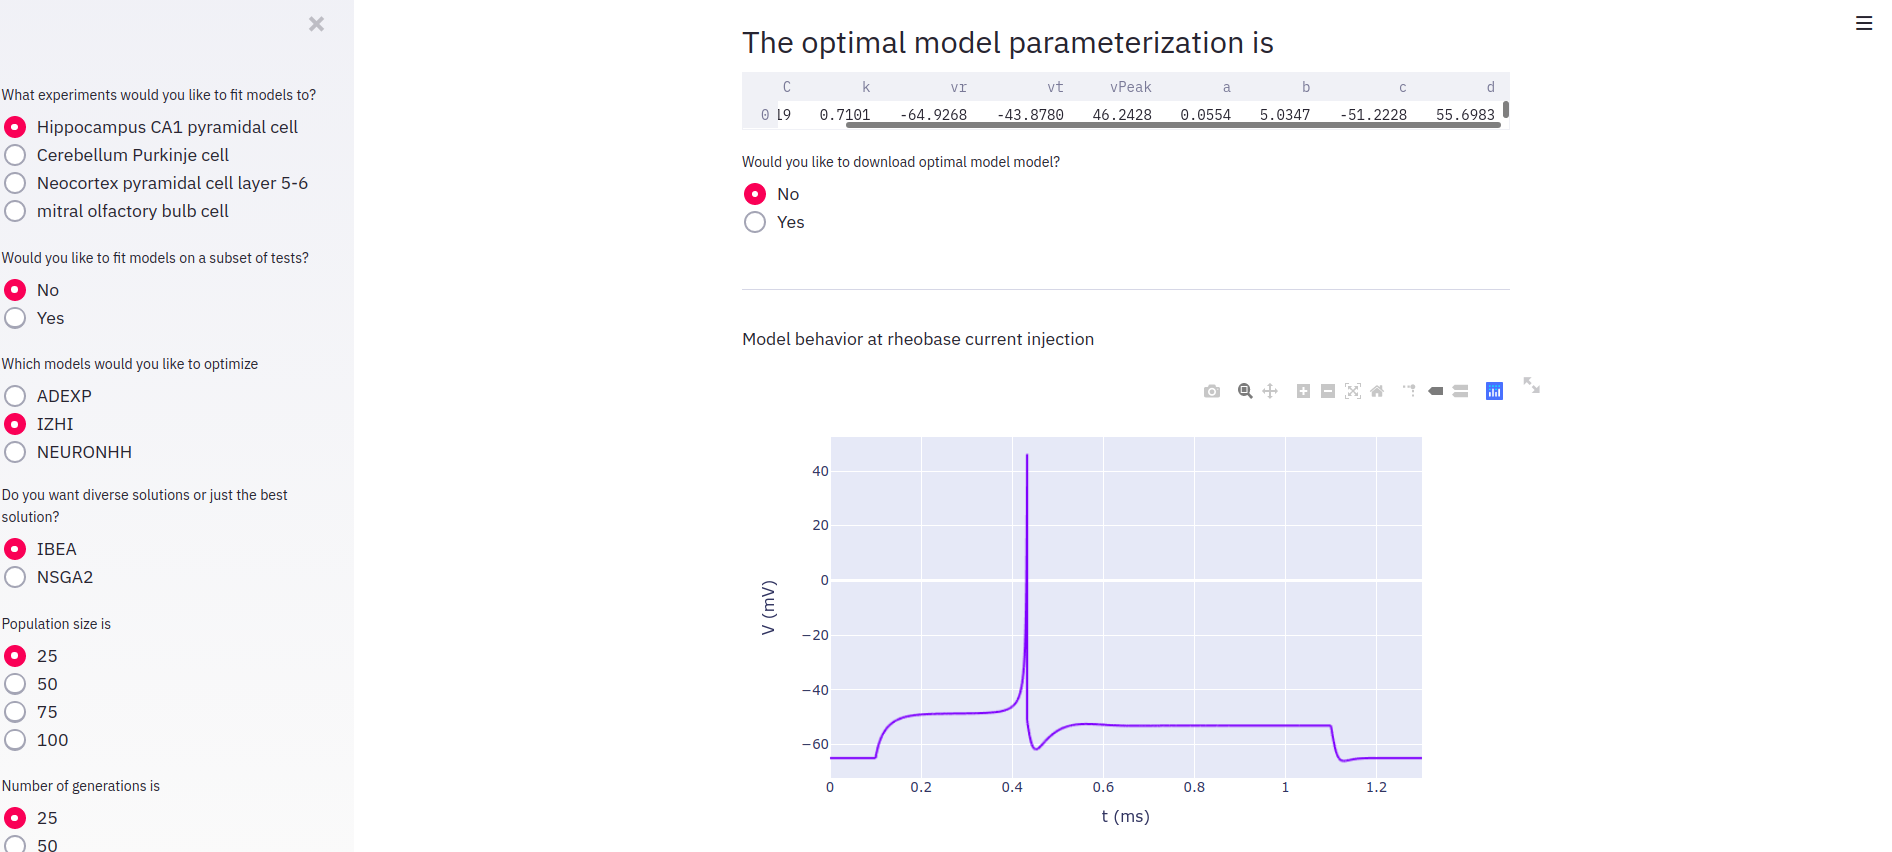
\includegraphics[scale=1]{chapters/app_tex/more_app_results}
\end{center}

\end{figure}

An accompanying interactive visualisation of the optimized model neuron firing under rheobase firing, and also under passive conditions is supplied.
\begin{figure}
\begin{center}

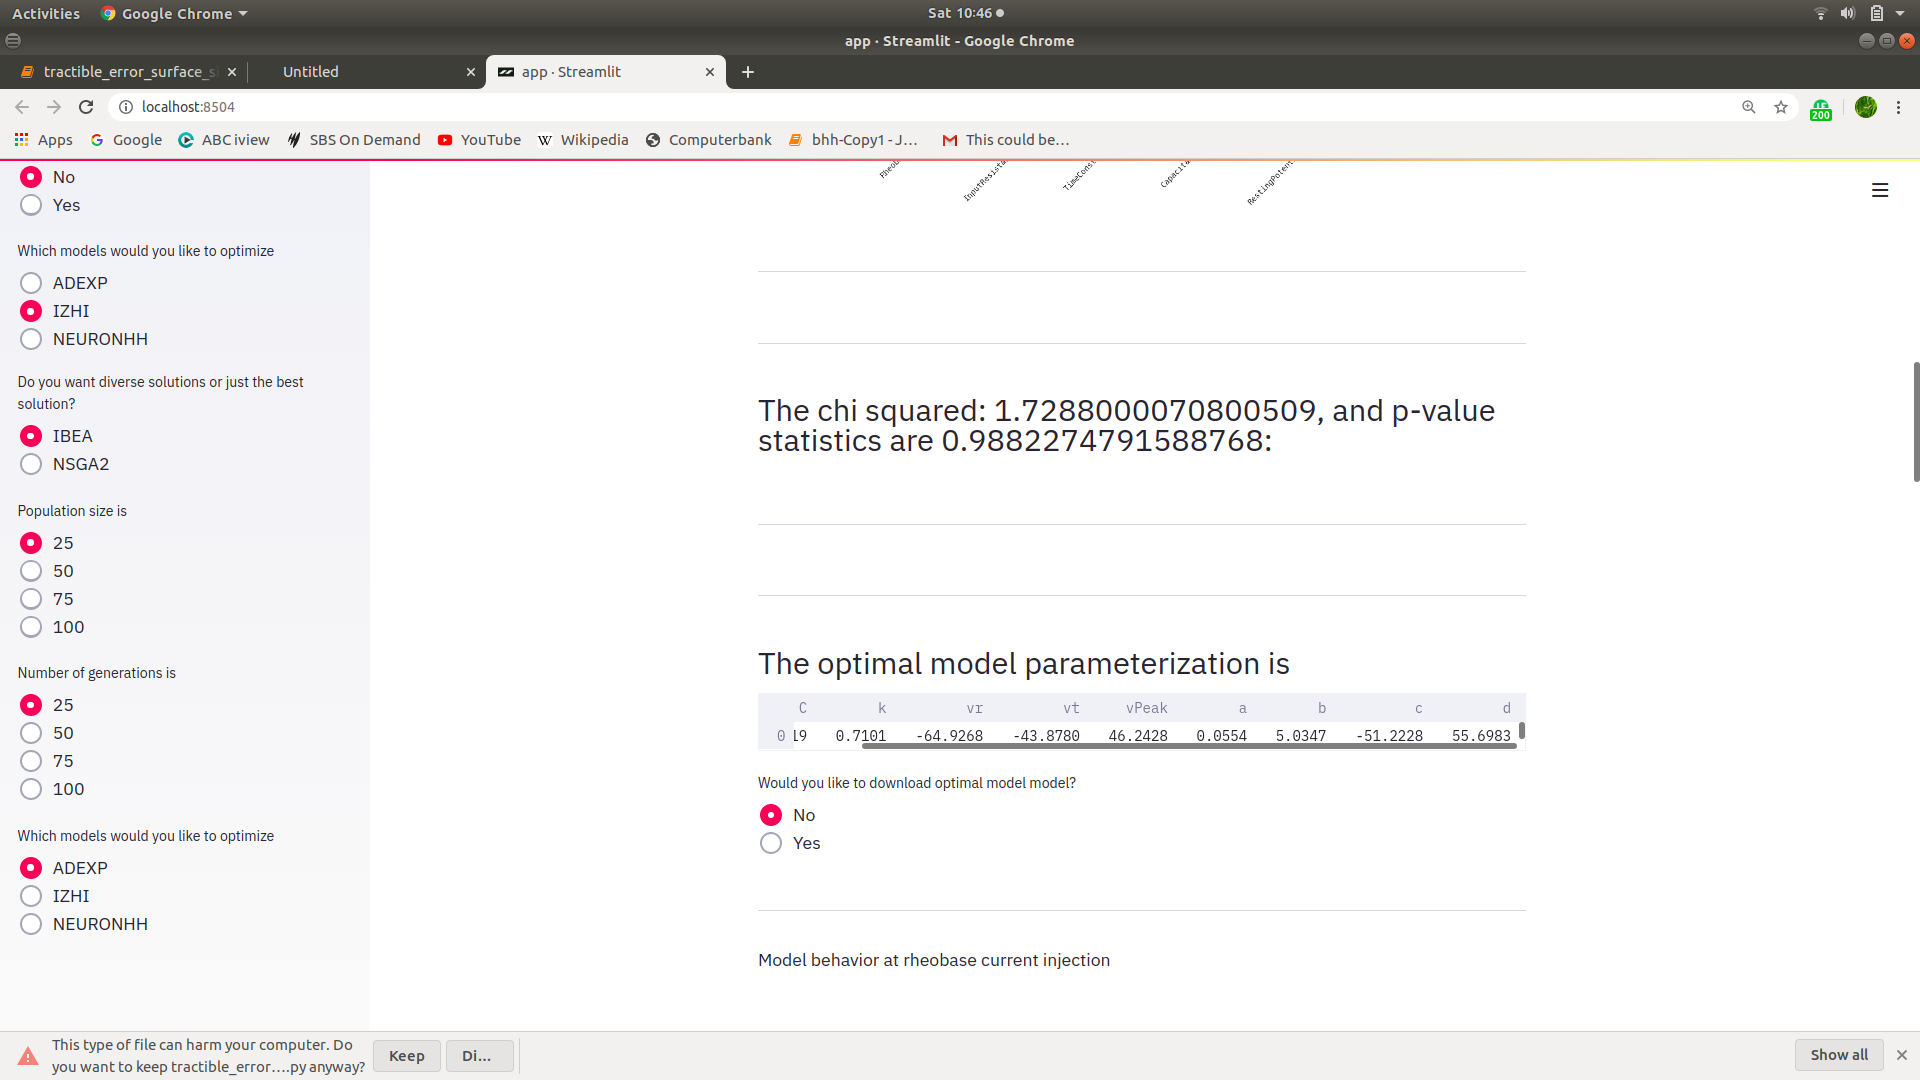
\includegraphics[scale=1]{chapters/app_tex/Screenshot from 2020-09-19 10-46-32}
\end{center}

\end{figure}


For each sciunit score in a suite, the Z-scores are visualized as an appropriately placed point on a bell curve. In addition to the $\chi^{2}$ test, this enables users to see how well the model does per test, on features that they may care more about.

The user then has the option of consulting displayed Z-scores, for each test.
\begin{figure}
\begin{center}
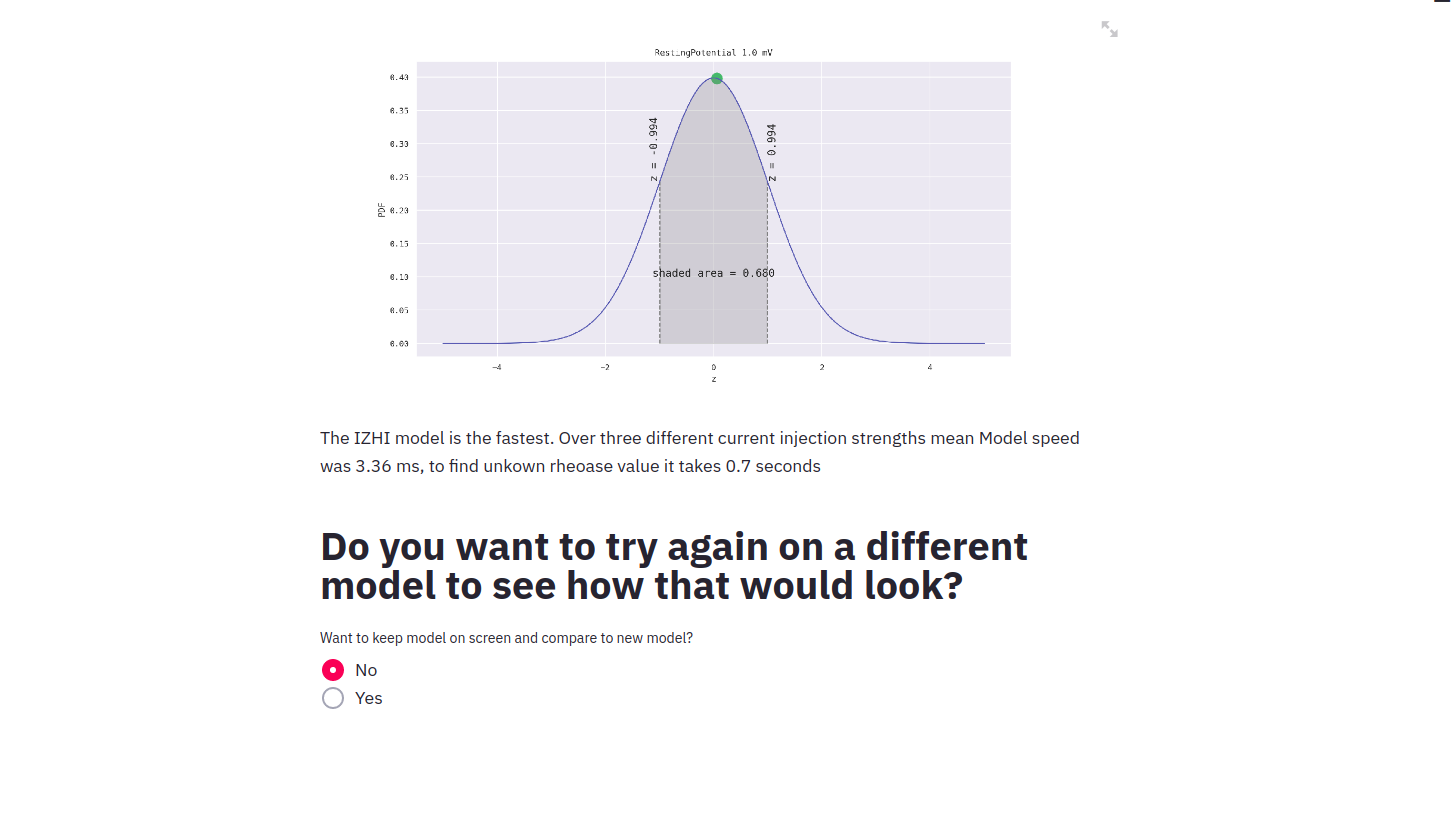
\includegraphics[scale=1]{chapters/app_tex/Screenshot from 2020-09-19 10-47-27}
\caption{In principle the web application is compatible with the approach of fitting models to the supra threshold multi-spiking experiments approach but this functionality does not exist at the time of writing}
\end{center}

\end{figure}



%\includegraphics[]{chapters/app_tex/Screenshot\ from\ 2020-09-19\ 10-47-31}



% STILL NEEDS A FEW basic results, from the appendix
%
%Test combinations that worked and did not work.
%note move the majority to the appendix
%Moved to appendix, will move back specific results



\subsection{Section 3.11}
Tests that were not always amenable to optimization:
\begin{itemize}
\item ThresholdTest
\item SpikeHalfWidth
\item Spike Amplitude
\end{itemize}
as discussed previously this is because of a threshold measurement that differs between cells. This may be more of a problem in certain regions of model parameter space, but the problem was general, it occurred in multiple models.
%Aim 1A, write something about tests overall.
%Overall the some 
Tests of static electrical properties amenable to optimization:
\begin{itemize}
\item FISlopeTests
\item Rheobase
\item Capacitance
\item Input Resistance
\item Time Constant 
\end{itemize}
%, , , , test worked but was conflicted. The tests that did not work. This is somewhere else.

Tests that worked within optimization:
Via \emph{Elephant} toolchain: FITests, Rheobase, Capacitance, Input Resistance, Time Constant, Resting Membrane Potential.
Via. 

When optimizing in the supra threshold regime Druckmann used:
(1) spike rate; (2) an accommodation index; (3) latency to first spike;(4) average AP overshoot; (5)average depth of after hyperpolarization (AHP); 
(6) average AP width similar to Druckman, when optimizing in the supra threshold regime.
When optimizing with reduced models, I found that the those 6 measurements were not enough to tightly constrain a fit, and additional constraints were helpful. In this work a minimum of 12 constraints were typically used:
\emph{EFEL} tool chain:
\begin{itemize}
\item AHP_depth
\item all_ISI_values,
\item Spikecount (similar to rate)
\item adaptation_index
\item mean_AP_amplitude  
\item min_voltage_between_spikes
\item minimum_voltage
\item peak_voltage
\item spike_half_width
\item time_to_first_spike
\item time_to_last_spike
\item voltage_base
\end{itemize}
 
%
%note move the majority to the appendix
\subsection{Electrical Features Allen Experiment Features}
%\subsection{The Experimental Measurements}

 \subsection{471819401 AdExp} scores, agreement\begin{tabular}{lllll}
\toprule
{} & RheobaseTest & TimeConstantTest & RestingPotentialTest & InputResistanceTest \\
\midrule
observations &     190.0 pA &          13.8 ms &             -77.5 mV &       132.0 megaohm \\
predictions  &    188.96 pA &         14.55 ms &            -77.91 mV &      128.53 megaohm \\
Z-Scores     &            0 &             0.02 &                    0 &                0.02 \\
\bottomrule
\end{tabular}

\subsection{Electrical Features NeuroElectro Experiment Features}
%\subsection{The Experimental Measurements}

\begin{table}[ht]
\centering
\resizebox{\textwidth}{!}{
\begin{tabular}{lllll}
\toprule
name & Hippocampus CA1 pyramidal cell & Cerebellum Purkinje cell & Neocortex pyramidal cell layer 5-6 &      olfactory mitral cell \\ 
\midrule
RheobaseTest                   &                     189.24 pA &                680.79 pA &                          213.85 pA &          NaN \\
InputResistanceTest            &                    107.08 Mohm &              142.06 Mohm &                        120.67 Mohm &  130.08 Mohm \\
TimeConstantTest               &                        24.5 ms &                      NaN &                           15.73 ms &     24.48 ms \\
CapacitanceTest                &                        89.8 pF &                620.27 pF &                          150.58 pF &    235.75 pF \\
RestingPotentialTest           &                      -65.23 mV &                -61.59 mV &                          -68.25 mV &    -58.14 mV \\
APWidthTest     &                        1.32 ms &                  0.41 ms &                            1.21 ms &      1.61 ms \\
APAmplitudeTest &                       86.36 mV &                 71.23 mV &                           80.44 mV &      68.4 mV \\
APThresholdTest &                       -47.6 mV &                -46.89 mV &                          -42.74 mV &     -38.9 mV \\
\bottomrule
\end{tabular}}
\end{table} 

\begin{table}[ht]
\centering
\resizebox{\textwidth}{!}{
\begin{tabular}{lllll}
\toprule
name & Hippocampus CA1 pyramidal cell & Cerebellum Purkinje cell & Neocortex pyramidal cell layer 5-6 &      olf\_mit \\
\midrule
RheobaseTest                   &                      189.24 pA &                680.79 pA &                          213.85 pA &          NaN \\
InputResistanceTest            &                    107.08 Mohm &              142.06 Mohm &                        120.67 Mohm &  130.08 Mohm \\
TimeConstantTest               &                        24.5 ms &                      NaN &                           15.73 ms &     24.48 ms \\
CapacitanceTest                &                        89.8 pF &                620.27 pF &                          150.58 pF &    235.75 pF \\
RestingPotentialTest           &                      -65.23 mV &                -61.59 mV &                          -68.25 mV &    -58.14 mV \\
InjectedCurrentAPWidthTest     &                        1.32 ms &                  0.41 ms &                            1.21 ms &      1.61 ms \\
InjectedCurrentAPAmplitudeTest &                       86.36 mV &                 71.23 mV &                           80.44 mV &      68.4 mV \\
InjectedCurrentAPThresholdTest &                       -47.6 mV &                -46.89 mV &                          -42.74 mV &     -38.9 mV \\
\bottomrule
\end{tabular}}
\end{table}

\subsection{Neocortex pyramidal cell layer 5-6, Izhikevich Model}
$\chi^{2}$
\begin{tabular}{lr}
\toprule
{} &         0 \\
\midrule
chi\_square &  1.976320 \\
p\_value    &  0.981729 \\
\bottomrule

\end{tabular}

\begin{table}[ht]
\centering
\resizebox{\textwidth}{!}{
\begin{tabular}{llll}
\toprule
{} & observations &    predictions & Z-Scores \\
\midrule
RheobaseTest                   &    213.85 pA &       45.04 pA &     1.13 \\
InputResistanceTest            &  120.67 Mohm &  84.48 megaohm &     0.44 \\
TimeConstantTest               &     15.73 ms &       12.28 ms &     0.45 \\
CapacitanceTest                &    150.58 pF &      145.41 pF &     0.03 \\
RestingPotentialTest           &    -68.25 mV &      -68.35 mV &     0.01 \\
InjectedCurrentAPWidthTest     &      1.21 ms &        1.31 ms &     0.16 \\
InjectedCurrentAPAmplitudeTest &     80.44 mV &        80.5 mV &        0 \\
InjectedCurrentAPThresholdTest &    -42.74 mV &      -38.51 mV &     0.51 \\
\bottomrule
\end{tabular}}
\end{table}

\subsection{Hippocampus CA1 pyramidal cell, Izhikevich Model}
$\chi^{2}$
\begin{tabular}{lrr}
\toprule
{} &  chi\_square &   p\_value \\
\midrule
0 &    2.125091 &  0.976935 \\
\bottomrule
\end{tabular}

\begin{table}[ht]
\centering
\resizebox{\textwidth}{!}{
\begin{tabular}{llll}
\toprule
{} & observations &    predictions & Z-Scores \\
\midrule
RheobaseTest                   &    189.24 pA &       32.24 pA &     0.54 \\
InputResistanceTest            &  107.08 Mohm &  97.76 megaohm &      0.1 \\
TimeConstantTest               &      24.5 ms &         9.6 ms &     0.72 \\
CapacitanceTest                &      89.8 pF &       98.24 pF &     0.13 \\
RestingPotentialTest           &    -65.23 mV &      -65.56 mV &     0.06 \\
InjectedCurrentAPWidthTest     &      1.32 ms &         1.2 ms &     0.17 \\
InjectedCurrentAPAmplitudeTest &     86.36 mV &       86.97 mV &     0.04 \\
InjectedCurrentAPThresholdTest &     -47.6 mV &       -40.0 mV &     1.12 \\
\bottomrule
\end{tabular}}
\end{table}

\subsection{Hippocampus CA1 pyramidal cell, Conductance Model}
$\chi^{2}$
\begin{tabular}{lrr}
\toprule
{} &  chi\_square &   p\_value \\
\midrule
0 &   17.216463 &  0.027932 \\
\bottomrule
\end{tabular}

\begin{table}[ht]
\centering
\resizebox{\textwidth}{!}{
\begin{tabular}{llll}
\toprule
{} & observations &     predictions & Z-Scores \\
\midrule
RheobaseTest                   &    189.24 pA &        225.0 pA &      0.1 \\
InputResistanceTest            &  107.08 Mohm &  130.26 megaohm &     0.27 \\
TimeConstantTest               &      24.5 ms &         6.52 ms &     0.91 \\
CapacitanceTest                &      89.8 pF &        50.05 pF &     0.78 \\
RestingPotentialTest           &    -65.23 mV &       -63.79 mV &     0.26 \\
InjectedCurrentAPWidthTest     &      1.32 ms &         0.25 ms &     2.54 \\
InjectedCurrentAPAmplitudeTest &     86.36 mV &        89.14 mV &      0.2 \\
InjectedCurrentAPThresholdTest &     -47.6 mV &       -62.83 mV &     3.02 \\
\bottomrule
\end{tabular}}
\end{table}

\subsection{Hippocampus CA1 pyramidal cell, Adaptive Exponential Model}
$\chi^{2}$
\begin{tabular}{lr}
\toprule
{} &          0 \\
\midrule
chi\_square &  10.232514 \\
p\_value    &   0.249084 \\
\bottomrule
\end{tabular}


\begin{table}[ht]
\centering
\resizebox{\textwidth}{!}{
\begin{tabular}{llll}
\toprule
{} & observations &     predictions & Z-Scores \\
\midrule
RheobaseTest                   &    189.24 pA &        225.0 pA &      0.1 \\
InputResistanceTest            &  107.08 Mohm &  130.26 megaohm &     0.27 \\
TimeConstantTest               &      24.5 ms &         6.52 ms &     0.91 \\
CapacitanceTest                &      89.8 pF &        50.05 pF &     0.78 \\
RestingPotentialTest           &    -65.23 mV &       -63.79 mV &     0.26 \\
InjectedCurrentAPWidthTest     &      1.32 ms &         0.25 ms &     2.54 \\
InjectedCurrentAPAmplitudeTest &     86.36 mV &        89.14 mV &      0.2 \\
InjectedCurrentAPThresholdTest &     -47.6 mV &       -62.83 mV &     3.02 \\
\bottomrule
\end{tabular}}
\end{table}

\subsection{Olfactory Mitral Cell Izhikevich Model}
\begin{table}[ht]
\centering
\resizebox{\textwidth}{!}{
\begin{tabular}{llll}
\toprule
{} & observations &     predictions & Z-Scores \\
\midrule
InputResistanceTest            &  130.08 Mohm &  111.76 megaohm &     0.21 \\
TimeConstantTest               &     24.48 ms &        26.35 ms &     0.18 \\
CapacitanceTest                &    235.75 pF &       235.77 pF &     0.03 \\
RestingPotentialTest           &    -58.14 mV &       -59.78 mV &      0.3 \\
InjectedCurrentAPWidthTest     &      1.61 ms &         1.54 ms &     0.19 \\
InjectedCurrentAPAmplitudeTest &      68.4 mV &        68.62 mV &     0.04 \\
InjectedCurrentAPThresholdTest &     -38.9 mV &       -30.45 mV &     1.35 \\
\bottomrule
\end{tabular}}
\end{table}
\subsubsection{Cerebellum Purkinje cell Experiment Conductance Izhikevich Model}\begin{tabular}{lr}
\toprule
{} &          0 \\
\midrule
chi\_square &  19.158050 \\
p\_value    &   0.014037 \\
\bottomrule
\end{tabular}
\begin{table}[ht]
\centering
\resizebox{\textwidth}{!}{
\begin{tabular}{llll}
\toprule
{} & observations &    predictions & Z-Scores \\
\midrule
RheobaseTest                   &    680.79 pA &        43.4 pA &     1.83 \\
InputResistanceTest            &  142.06 Mohm &  66.98 megaohm &     1.29 \\
CapacitanceTest                &    620.27 pF &       68.27 pF &     3.36 \\
RestingPotentialTest           &    -61.59 mV &      -61.61 mV &        0 \\
InjectedCurrentAPWidthTest     &      0.41 ms &        0.48 ms &     0.32 \\
InjectedCurrentAPAmplitudeTest &     71.23 mV &       71.41 mV &     0.01 \\
InjectedCurrentAPThresholdTest &    -46.89 mV &      -37.79 mV &     1.66 \\
\bottomrule
\end{tabular}}
\end{table}
%%\subsection{Neocortical Layer 4/5 Pyramidal Cell Test Suite}
\subsubsection{Performance of Layer 5 Prefrontal cortex Pyramidal Neuron on NeuronUnit tests of model data agreement}
\cite{van2016bluepyopt}
A suite of neuronunit tests containing the tests: rheobase value, membrane voltage time constant ($tau_{m})$, input resistance was computed. This multi-compartment, conductance based model served as a useful benchmark, for us to evaluate the relative performance of reduced model fits.

Significant development work went into making the model eligible to take NeuronUnit tests, by way of creating a specially dedicated NeuronUnit backend, to run this complicated conductance based multi-compartment model originating from the blue brain model \cite{markram2015reconstruction}.

This elaborate biophysical model includes the backpropogating dendritic action potential.
\url{}



\begin{figure}
\begin{center}


\centering
\begin{subfigure}{.2\textwidth}
  \centering
    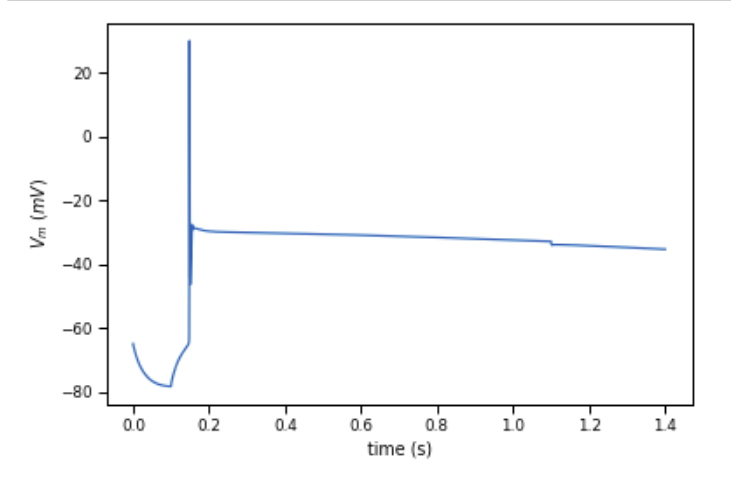
\includegraphics[scale=0.5]{figures/correct_active_l5pc.png}
    \caption{A current injection sufficient for causing a single spike is applied for a whole second from $100ms-1100ms$}
  \label{fig:sub1}
\end{subfigure}

\centering
\begin{subfigure}{.2\textwidth}
  \centering
    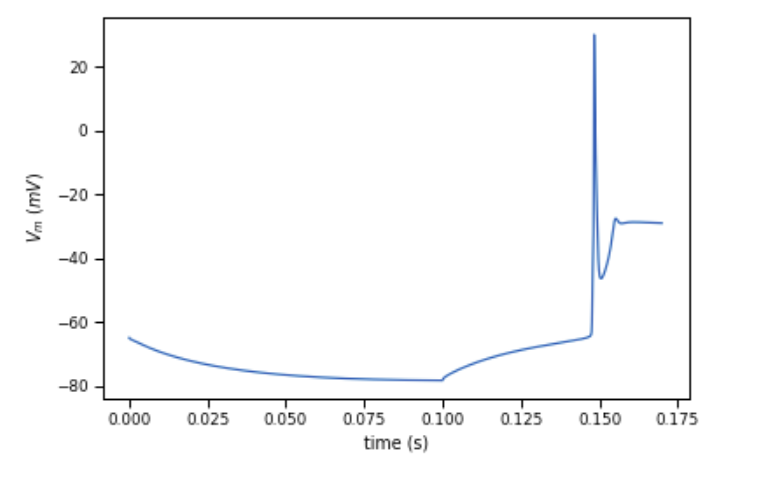
\includegraphics[scale=0.5]{figures/spike_shape.png}
    \caption{The spike shape is very brief in duration, and so it is worth zooming in for a closer look}
  \label{fig:sub1}
\end{subfigure}


\begin{subfigure}{.2\textwidth}
  \centering
    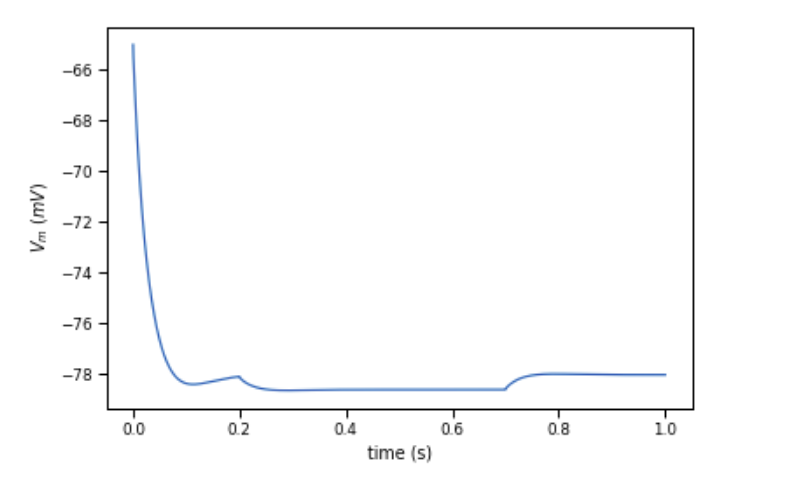
\includegraphics[scale=0.5]{figures/correct_passive_l5pc.png}
    \caption{A current injection value of -$10pA$ is applied to the cell for the duration of $200ms-700ms$}
  \label{fig:sub2}
\end{subfigure}
\label{fig:test}
\end{center}
\end{figure}


A test suite was constructed using NeuroElectro for the layer 4/5 Prefrontal Cortex pyramidal cell, and we were able to evaluate this layer 5 PC cells against the criteria of the neuroelectro test suite. 

\begin{table}[ht]
\centering
\resizebox{\textwidth}{!}{
\begin{tabular}{llll}
\toprule
{} & observations &   predictions & Z-Scores \\
\midrule
RheobaseTest                   &    213.85 pA &      225.0 pA &  0.06542 \\
InputResistanceTest            &  120.67 Mohm &  50.7 megaohm &  -0.9013 \\
TimeConstantTest               &     15.73 ms &      16.76 ms &   0.1409 \\
CapacitanceTest                &    150.58 pF &     330.66 pF &    1.289 \\
RestingPotentialTest           &    -68.25 mV &     -78.04 mV &   -1.499 \\
InjectedCurrentAPWidthTest     &      1.21 ms &       0.15 ms &   -1.979 \\
InjectedCurrentAPAmplitudeTest &     80.44 mV &      89.58 mV &   0.7174 \\
InjectedCurrentAPThresholdTest &    -42.74 mV &     -59.57 mV &   -2.094 \\
\bottomrule
\end{tabular}}
\end{table}
The corresponding statistics were
$(\chi^{2},p_{value})=(13.5609360364, 0.093951963105254)$

    
It is worth noting that the layer 5 neocortical pyramidal neuron was very slow to dispatch relative to the reduced models developed in this thesis work. Where as a typical reduced model described here evaluated in the order of $~0.0025 seconds$, this model on average took $5.74$, for a single run and $34.8$ to solve for the models Rheobase, current.


This model was pre-optimized to fit to spike times and F/I mainly, and so it should not necassarily be expected to fit other electrical charactersistics of the cell. Only the rheobase test, and the time constant test seemed to fall within the range of biological plausibility.
None the less, this model remains a useful benchmark for reduced neuronal models.
%
\subsection{Experiment Fitted Results Allen Brain Institute, Cell-types Ephysiological data, Elephant Tests}


\subsection{Experiment Fitted Results Neuroelectro data, Elephant Tests}

Over four different experiments we constructed 7-8 different NeuronUnit tests. 

$\chi^{2}=\Sigma zscores^{2} $

%https://en.wikipedia.org/wiki/Chi-square_distribution
%This allows you to state this as a hypothesis test with a p-value.  The chi-square statistic would simply be , and the p-value would be 1-scipy.stats.chi2.cdf(x, 8) where 8 is the number of elephant tests (and Z-scores).  A very small p-value (which would come from very large chi-square statistic, much larger than expected for random variation) %would mean the optimizer was less successful at recovering the true model.

See appendix:\ref{table:static_electrical_properties}
The Izhikevich Model and the Point Conductance Model were able to achieve high p-values, and small chi-squared statistics when seven or eight of the tests were considered together.

For example the Izhikevich model fitted to Hippocampus CA1 pyramidal cell data achieved $ (\chi^{2} ,p-value) =(2.1250913868824415, 0.9769347643323284) $

The olfactory Mitral cell
$ (\chi^{2} ,p-value) =(2.0190436240810925, 0.9804224622781068) $

and the cerebellum Purkinje cell. For contrast p-value and chi-squared statistics on the best random models were:

%(2.0190436240810925, 0.9804224622781068)r
\subsection{Data fitted Results on four different classes of model were only modestly good for the Izhikevich Model and the Point Conductance Model}

To make the argument that limitations in reduced neural models were the cause of modest model/experiment agreement, we first had to rule out alternative possibilities. One possibility was that the experimental measurements were faulty, and that the measurements were possibly spurious because of in appropriate averaging. It was found that mainly the olfactory bulb mitral cell was prone to having underlying bi-modal data distributions, and this was especially true for resting membrane

that the models shouldn't be able to reproduce. When considering the data sources, the methods of data collection and data quality should be reliable, the one main 

we first needed to exclude the possibility that there might be something wrong with the data, we are fitting models to.

We needed to rule out was that the data sources did not reflect bi-modal distributions, since the neuroelectro data was the actually the mean over different laboratories, animals, and recording epochs. The mean of a population can often be a robust representation of a population, however there are circumstances when the opposite is true, such as when the underlying data is generated by two different processes, leading to bimodal distributions. Fortunately, it is not hard to test if experimental data, has an underlying bimodal distribution. That test was performed using human judgement for all measurements that were used to fit the model to experiments. Except in the case of the Allen Brain data, because the Allen Brain data consisted of individual raw experiments, and population averaging did not apply. For measurements used in the elephant optimization pipeline.

Below I show distributions for  Time Constant, Input Resistance, Capacitance, Rheobase, Resting Membrane Potential, bimodal distributions did not apply, so we could rule out inaccurate data as a reason for poor model performance.

There is no reason to believe that reduced neural models could not be made to fit inaccurate neural recordings as well as real ones, if the fiction is just caused by noise, then it is still possible that hypothetical spurious values would still be in reach of the Izhikevich model. The izhikevich model can be made to generate some physiologically implausible waveform shapes. 
% a different question, of are the models arbitary waveform generators? 

Besides even if the data was wrong, it wouldn't necessarily follow that models couldn't reproduce the inaccurate data. Instead what we see is, that models can fit one type of experimental measurement at a time, but they can't fit all measurements at once. This result suggests that model flexibility is the most fundamental cause of modest, model experiment disagreement.


%In light of this result, one might ask, i
If reduced models are not excellent at fitting data, are brain simulations really that much more realistic, when we use data driven fitted models in the place of generic model parameters? If data driven model fits lead to models that fit one measurement better than others, which fitness criteria will lead to the greatest consequence for network simulations?

%to answer that question we have created some large




\section{Limitations data we were using was of Existing Approaches} 
Existing community supported simulated models were problem ridden, and our own custom methods were used as work arounds.

% NEURON version of Izhi model is not as fast as one might expect, this may because of the way we tried to implement the model, by creating and destroying HOC module instances, that contain the model. 

%A
% Nonetheless, 
At first we accessed an implementation of the Izhikevich model that was translated from jNEUROML into a NEURON simulator implementation. The problem with this implementation is that it had fragmented the whole Izhikevich model into chattering and non chattering subtypes. The model implementation seemed to have an internal conflict between two capacitive terms. The problem was that the Izhikevich model requires only one capacitive term.

implemented in NEURON which was derived from a J-NeuroML translation, could not reproduce all of the Izhi original publication figures, because it had two different conflicting sources of capacitance.\\
\\
From J-NeuroML we created NEURON version of Izhikich model, however we were not able to make this model execution times brief enough to be useful for optimization. Although the NEURON simulator is designed to be fast, their may be a cost associated with reloading the NEURON environment many times in fast succession.

This should not go in the general introduction, but in the intro to the appropriate section of the results where you use those models.
%Test combinations that worked and did not work.
%note move the majority to the appendix
%Moved to appendix, will move back specific results
% Put some of the below (whatever is worthwhile) into Results section 1b




%    2a. First just do basic ones (like Izhikevich) for a few cell types, then you can close with L5PC.
%    2b. The app (which supports 2a).

% The optimized models part of this section is predicated on result 1b (so that optimization results can be believed).  You already have the poster for this. I think this captures most of your results in three themes.  Other results which are really methods, like parallel rheobase search, can stay in the methods, and you will get credit for them there.


% , although some pre-existing APIs already existed, I needed to write new ones.  This is in a sense a method, but you can still report that these tests are runnable, even outside of optimization.
 %Why (briefly, saving some for discussion)?  NeuroElectro vs Allen also belong here, and fits in with 1a.  You should talk about model means vs means of models (or whatever we are calling it) 
       
  %here, if you have the results for it or think you can in 3 weeks.  
       %You can talk about rippled error surfaces — this is such a deep technical detail that I wouldn’t spend a lot of time on it.  In other words it may be important but it will be almost impossible to follow even if written well.
